\documentclass{uwstat572}

\usepackage{graphicx}
\usepackage{subcaption}
\usepackage{float}
\usepackage{ulem}
\usepackage{color}
\usepackage{natbib}
\usepackage{amsmath}
\usepackage{lipsum}

%%\setlength{\oddsidemargin}{0.25in}
%%\setlength{\textwidth}{6in}
%%\setlength{\topmargin}{0.5in}
%%\setlength{\textheight}{9in}

\renewcommand{\baselinestretch}{1.5} 

\newcommand{\vmdel}[1]{\sout{#1}}
\newcommand{\vmadd}[1]{\textbf{\color{red}{#1}}}
\newcommand{\vmcomment}[1]{({\color{blue}{VM's comment:}} \textbf{\color{blue}{#1}})}

\bibliographystyle{apalike}

\begin{document}
%%\maketitle

\begin{center}
  {\LARGE Statistical Inference and Computational Efficiency for Spatial Infectious Disease Models with Plantation Data}\\\ \\
  {Nathan Welch \\ 
    Department of Statistics, University of Washington Seattle, WA, 98195, USA
  }
\end{center}

\begin{abstract}
This paper aims to conduct statistical inference for parameters of an individual level infectious disease model. 
Individual level models have the capacity to reflect spatial and temporal influences on disease propagation among infected and susceptible individuals.
A simple individual level model is derived and fit to data collected during an insect infestation of a sugar cane field.
Model parameters are estimated using the Metropolis sampling algorithm; however, the computational burden created by fitting even a simple model leads to prohibitively long computation times. 
\textit{Statistical inference and computational efficiency for spatial infectious disease models with plantation data} \citep{Brown} fit a model to the same data. 
The authors offer mathematical and computational insights to improve computation time, but errors in the published Metropolis algorithm source code led the authors to inferences and conclusions unsupportable with the data alone. 
\end{abstract}

\section{Introduction}

Disease propagation modeling is an expansive and active area of mathematical research \citep{Kranz, Anderson}.
Statistical inference for parameters underlying these models is less mature, but computational advances in recent years make it possible to encode convoluted dependencies and draw inference on the parameters influencing disease propagation. 
Improving our understanding of these parameters will lead to more effective responses or interventions to disease outbreaks. 

\citet{Brown} set out to conduct statistical inference for a simple class of disease propagation models by estimating the risk that a susceptible individual contracts a disease from an infected member of the population. 
In these models, the risk of contracting the disease is modeled at the individual level rather than for the population as a whole. 
The goal is to formulate models that reflect changes in individual risk that correspond to the number of the infected individuals, their proximity to susceptible members of the population, and the duration a susceptible individuals  exposure to those infected. 
While this model is conceptually convenient, the computational complexity and limitations of algorithms capable of fitting such a model create significant challenges.
In \citet{Brown}, the authors appeal to standard likelihood methods and the Metropolis algorithm \citep{Metropolis} to estimate the parameters of a simple individual level model (ILM) for disease propagation.
The emphasis on basic components like the Metropolis sampler and simple disease model focuses readers on common challenges inherent with data for statistical inference with infectious disease data. 

\subsection{Literature Review}
\label{literature_review}
\citet{Haber} introduced ILMs in the context of disease spread among members within households. 
This early ILM assumes infected individuals are dispersed evenly throughout the population. 
It also assumes complete data are available to fit these early models. 
\citet{Becker} surveys a number of models and the types of data sets these models can accommodate. 
His work highlights the distinction between studying disease spread from a mathematical perspective as apposed to a statistical inference point of view and summarizes the principle challenges that disease propagation presents to many statistical methods.

\citet{ONeill} builds on the idea that one does not have to choose between parameter inference and mathematical insight. 
In fact, the authors show that a basic Metropolis-Hastings algorithm clears the way for more realistic modeling assumptions and interdependencies. 
\citet{Jewell} provides an updated perspective and outlines several MCMC design patterns for convoluted models.
\citet{Brown} primarily contributes another example of these methods along with computational efficiencies beyond an MCMC framework. 

While improved computation power made it possible to fit more complex statistical disease models, evaluating likelihood functions that include spatio-temporal components becomes challenging when there are more than a few observations. 
As the cost to evaluate the likelihood function grows with the number of observations, the utility of MCMC approaches declines.
\citet{McKinley} proposes Approximately Bayesian Computation (ABC) that avoids calculating the likelihood by generating an approximation to the likelihood function with each pass through an MCMC implementation. 
\citet{Diggle} forgoes the complexity of full likelihood inference and instead appeals to the partial likelihood function to carry out inference for the parameters of interest. 
\citet{Deardon} uses a Taylor series to approximate infection kernel function to make a Bayesian approach computationally practical. 
These methods led to reduced computation times compared to a full MCMC implementation, but each either require either completely observed data or are too closely associated with a particular model to be widely applicable.

\subsection{Statistical Problem}
Contemplating the complexity of statistical inference for an individual level infectious disease model whose infection rates include spatial and temporal dependencies is daunting.
However, modeling disease propagation among regularly spaced crops on a farm reduces the challenge. 
This study aims to conduct statistical inference for an ILM fit to an insect infestation of a Guadeloupe sugar cane field over a period of 30 weeks.
Figure \ref{fig:data_plot} summarizes the sugar cane data set. 
The black dots indicate locations of infected plants at the conclusion of the 30 week study period. 
Grey dots indicate the location of plants that were not infected. 
The plot on the right shows the cumulative number of infected plants after each inspection.

\begin{figure}[h]
	\centering
	\begin{subfigure}[b]{0.49\textwidth}
		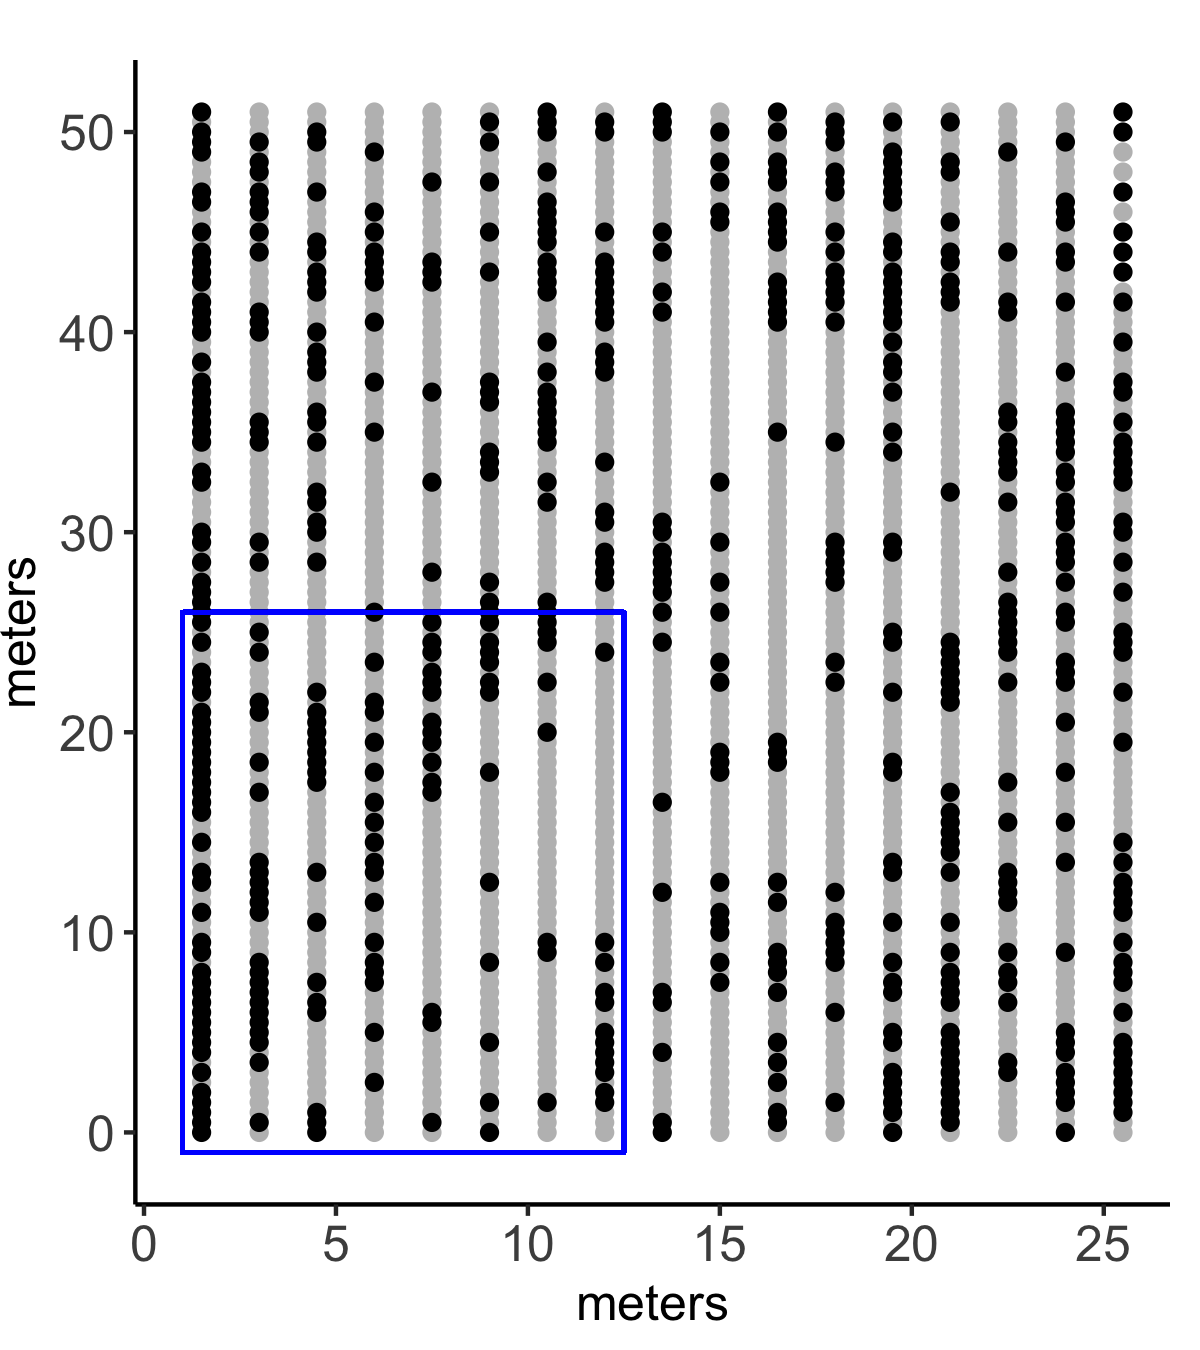
\includegraphics[width=\textwidth]{figures/figure_1a.png}
		\caption{}
		\label{fig:plants}
	\end{subfigure}
	\hfill
	\begin{subfigure}[b]{0.49\textwidth}
		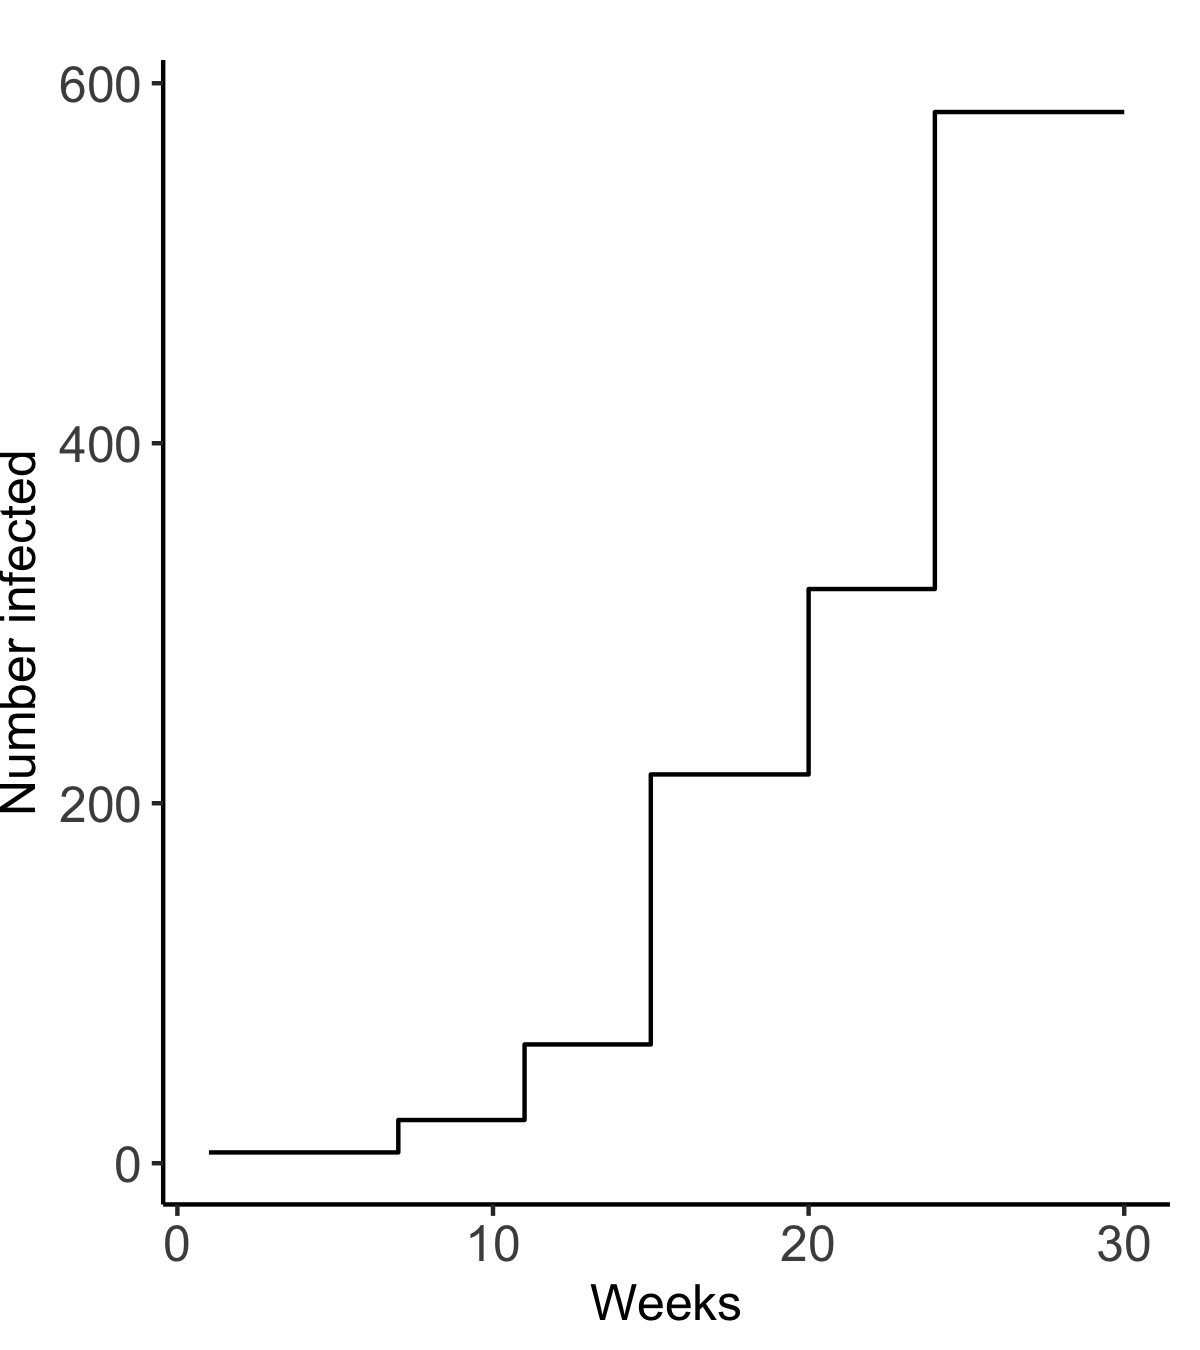
\includegraphics[width=\textwidth]{figures/figure_1b.png}
		\caption{}
		\label{fig:cum_infection}
	\end{subfigure}
	\caption{(\subref{fig:plants}) Plant locations (meters) and infection status (black=infected) after 30 weeks; (\subref{fig:cum_infection}) number of infected plants at each inspection time}
	\label{fig:data_plot}
\end{figure} 

When modeling disease propagation among individuals who are either susceptible or already infected, the time of infection and duration of susceptible individuals' exposures to infected members of the population are critical. 
These data are necessary to infer the rate at which the disease moves from the infected to the susceptible; however, infection times are rarely--if ever--known to any reliable level of precision. 
Even extremely dangerous or damaging diseases among closely monitored populations such as foot and mouth disease among livestock lack granular infection time data \citep{Diggle, Deardon}. 
As a result, plausible inference methods must include some means to account for uncertainty in infection times. 

The sugar cane data set includes the infection status of 1,742 plants at six times over a 30 week period. 
Each observation lists the plant location on a two-dimensional rectangular grid and whether it is infected at week 0, 6, 10, 14, 19, 23, and 30.
For this data set, it is reasonable to assume that once a plant becomes infected, it remains infected for the duration of the study period. 
A Susceptible-Infected (SI) model is appropriate for this situation and \citet{Jewell} provides a thorough introduction to this and other disease model frameworks. 
While an SI model is particularly simple, the model is plausible considering the way that an infestation proceeds for an aphid infestation of plants over 30 weeks time. 
Starting with a simple model also emphasizes the principle statistical components handled by \citet{Brown}, e.g. unknown infection times. 

Intervals in which susceptible plants became infected are recorded, but the data do not include granular infection time data.  
As a result, there is no way of knowing how long a plant occupied the susceptible and infected stages.
This is a common experimental design, and the details of studies that include this \textit{Type I censoring} with \textit{right} and \textit{interval censored} data are discussed at length in survival analysis texts such as \citet{Klein}. 
While the data collection framework in \citet{Brown} is standard, inference methods for \textit{interval censored} modeling parameters remains more nuanced.

Data augmentation is a common approach to overcoming this inference with unknown infection times. 
In this case, unknown infection times are modeled as latent variables. 
Including these latent variables makes the likelihood function tractable, but inflating the parameter space complicates the model fitting process. 
These factors point to a Bayesian approach to approximating the posterior parameter space of the SI model. 
\citet{Jewell} discusses an augmentation approach in the context of a \textit{Metropolis-in-Gibbs} MCMC framework and the simulation setup described in the next section follows directly. 

\section{Methods}
\subsection{Model and Likelihood}

Inference for ILM model parameters begins with the likelihood function. 
Plausible models account for the locations of infected and susceptible plants along with the respective infection times and durations of exposures. 
However, time intervals in which a susceptible plant becomes infected are the only temporal information in the data. 
As a result, treat the infection time, $\tau_j$, for plant $j$ as a latent variable. 
While this approach significantly expands the parameter space, it also leads to a tractable likelihood function. 
Note too that the latent variable domains are restricted to the time periods in which each individual's infection status changed. 

The model must also account for the transmission rate differential induced by the physical distance separating infected and susceptible plants. 
The transmission rate between an infected plant far from a susceptible plant should be smaller than the rate between two plants next to one another.
As a result, let the function $\theta f(x_i -x_j \sigma | \sigma)$ denote the rate of infection for plant $i$ at time $t$ after plant $j$ was infected prior to $t$. 
After including a term capturing the rate of spontaneous infection, $\mu$, the hazard function at plant $i$ and time $t$ given the infection times for plants $j \in \{1, 2, \dots, 1742\}$ is 
$$\lambda(x_i,t) = \mu + \sum_{j; \tau_j<t} \theta \, f(x_i - x_j; \sigma)$$
Now consider the contribution that plant $x_i$ makes to the likelihood if it is infected at time $0<\tau_i<T=30$ weeks. 
By definition of the hazard function, the instantaneous infection rate at plant $x_i$ is
\begin{align*}
\lambda(x_i, t) &= \lim_{dt \to 0} \frac{Pr\{ t \le \tau_i < t+dt | \tau_i \ge t \}}{dt} \\
	&= \lim_{dt \to 0} \frac{Pr\{ t \le \tau_i < t+dt\}}{Pr\{\tau_i\ge t\}dt}\\
	&= \lim_{dt \to 0} \frac{F_i(t+dt) - F_i(t)}{(1-F_i(t))dt} \\
	&= \frac{f_i(t)}{S_i(t)}\\
	&= -\frac{d}{dt} \log S_i(t) \\
\implies S_i(t) &= \exp \left\{ - \int_0^t \lambda(x_i,s) ds  \right\} = \exp \left\{ - \Lambda_i(t)  \right\}
\end{align*}
where $S_i$, $f_i$, and $\Lambda_i$ denote the respective survival function, probability distribution function (pdf), and cumulative hazard for plant $x_i$. 
From this expression, it follows that
$$ f_i(t) = \lambda(x_i,t) \exp \left\{ - \int_0^t \lambda(x_i,t) dt  \right\}$$
establishing the pdf that plant $x_i$ contributes to the likelihood function if $t<T=30$ weeks. 
Plants that remain healthy throughout the study period contribute $S_i(t)$ to the likelihood. 
As a result, the complete likelihood function is
\begin{equation} 
L(\theta, \mu, \tau) = \left[ \prod_{i;\tau_i \le T} \exp \left\{-\int^{\tau_i}_0 \lambda(x_i, t)dt\right \} \lambda(x_i, \tau_i)\right] \left[ \prod_{i;\tau_i > T} \exp \left\{-\int^{\tau_i}_0 \lambda(x_i, t)dt \right\}\right] 
\end{equation}

The last component of the model to specify is the kernel function, $f(x_i -x_j | \sigma)$. 
In this case, a radially symmetric bivariate Gaussian density is appropriate. 
\begin{equation} f( x_i-x_j |\sigma) = \frac{1}{2\pi \sigma^2} \exp \left\{-\frac{ ||x_i-x_j||^2}{2\sigma^2} \right\} \label{eq:kernel} \end{equation}
The Gaussian kernel is physically reasonable since the movement of aphids among plants can be modeled by Brownian Motion. 
With this argument, $\sigma^2$ in (\ref{eq:kernel}) denotes the variance of the distance an aphid travels in one week. 

\subsection{Prior Distributions}
\citet{Brown} suggests weakly informative priors for the endemic infection rate ($\mu$), the epidemic infection rate ($\theta$), and the standard deviation for distance disease traveled in a week ($\sigma$). 
These distributions were based on 95\% prior prediction intervals for each parameter. 
While the authors suggested an approach to specifying the hyperparameters for each variable, the following sections explicitly workout the details for the $\mu$ and $\theta$ prior. 
Multiple approaches were devised to derive the $\sigma$ prior hyperparameters; however, it was not possible to derive the results for this parameter based on the method published in the paper. 

\subsubsection{$\boldsymbol{\mu}$ Prior Predictive Distribution Specification}
The endemic infection rate influences the number of spontaneous infections over a specified time period. 
While spontaneously infected plants have the capacity to produce new infections, consider the case where only endemic infections are possible.
If epidemic infections are not possible, then each of the 583 infections recorded over the 30 week study period could be modeled by a constant endemic infection rate. 
Assuming 1 infection at the 2.5\% quantile and 630 at 97.5\%, it is possible to solve for the hyperparameters of $\mu \sim \Gamma(\alpha, \beta)$. 

The probability of observing $k$ infections under the prior predictive distribution is
\begin{equation}
P(k) = \int_0^{\infty} P(k, \mu) d\mu = \int_0^{\infty} P(k \mid \mu)  P(\mu) d\mu
\label{eq:prior_predictive}
\end{equation}
Note that while only the first infection is recorded, it is possible for plants to be infected multiple times. 
This realization suggests the sampling model $k \mid \mu \sim$ Poisson($\mu$) is not only convenient, but also appropriate. 
Therefore, if $\mu \sim \Gamma(\alpha, \beta)$,
\begin{align*}
P(k) &= \int_0^{\infty} \frac{\mu^k e^{\mu}}{k!}  \frac{\beta^{\alpha}}{\Gamma(\alpha)} \mu^{\alpha - 1} e^{-\beta \mu}d\mu \\
	&= \frac{\beta^{\alpha} \Gamma(\alpha+k)}{k! \; \Gamma(\alpha) \; (1+\beta)^{\alpha+k}}  \int_0^{\infty} \frac{(1+\beta)^{\alpha+k}}{\Gamma(\alpha+k)} \mu^{\alpha + k - 1} e^{-(1+\beta)\mu}d\mu \\
	&= \frac{\Gamma(\alpha+k)}{\Gamma(k+1) \Gamma(\alpha)} \left( \frac{\beta}{1+\beta} \right)^{\alpha} \left( \frac{1}{1+\beta} \right)^k
\end{align*}
Now consider the 2.5\% and 97.5\% quantiles for this distribution. 
\begin{align*}
P(k=0) &= \left( \frac{\beta}{1+\beta} \right)^{\alpha} \\
P(k \ge N) &= \sum_{k=N}^{\infty} \frac{\Gamma(\alpha+k)}{\Gamma(k+1) \Gamma(\alpha)} \left( \frac{\beta}{1+\beta} \right)^{\alpha} \left( \frac{1}{1+\beta} \right)^k \\
	&=1 - \sum_{k=0}^{N-1} \frac{\Gamma(\alpha+k)}{\Gamma(k+1) \Gamma(\alpha)} \left( \frac{\beta}{1+\beta} \right)^{\alpha} \left( \frac{1}{1+\beta} \right)^k 
\end{align*}
where $N=630$ for the full data set. 
Substituting $P(k=0)=P(k \ge N)=0.025$, it follows that 
\begin{align*}
\alpha &= \frac{\log 0.025}{\log \left( \frac{\beta}{\beta+1} \right)} \\
0 &= \sum_{k=0}^{N-1} \exp \left\{ \log \Gamma(\alpha+k) - \log \Gamma(k+1) - \log \Gamma(\alpha) + \alpha \log \left(\frac{\beta}{\beta +1} \right) + x \log \left(\frac{1}{\beta +1} \right) \right\} - 0.975
\end{align*}
Plugging these equations into a numerical solver with $N=630$ leads to $\alpha=0.6893886$ and $\beta=0.004766281$. 
These results are consistent with \citet{Brown}'s findings, i.e. $\alpha=0.7$ and $\beta=0.004$. 
However, these small differences do change the quantiles and variances corresponding to the distribution $\mu_{\text{Brown}} \sim \Gamma(0.7, 0.004)$ and $\mu_{\text{replicated}} \sim \Gamma(0.6893886, 0.004766281)$. 
Table \ref{table:mu_prior_quantile} shows the quantiles, means, and variances for the prior predictive distribution for $\mu$. 

\begin{table}[ht]
\centering
\begin{tabular}{rrrrr}
  \hline
 & 2.5\% & 97.5\% & mean & variance \\ 
  \hline
Brown et. al. & 1.12 & 755.06 & 175.00 & 43750.00 \\ 
  Replicated & 0.87 & 628.35 & 144.64 & 30346.23 \\ 
   \hline
\end{tabular}
\caption{$\mu$ prior predictive distribution properties for the distribution reported by \cite{Brown} compared to the distribution replicated by following the specification procedure described}
\label{table:mu_prior_quantile}
\end{table}

While the replicated parameter values for $\alpha$ and $\beta$ in the priors are consistent with the results reported in \citep{Brown}, $\alpha=0.7$ and $\beta=0.004$ leads to 755.06 at the 97.5\% quantile instead of 630 suggested in the derivation method described. 
The approach described by the authors also leads to a slightly more informative prior based on the variances of the two distributions. 

Each of the priors are important to inference, but correctly formulating the prior for $\mu$ is critical. 
If $\mu$ is too low, then there is no way for an epidemic to emerge within a field of susceptible plants. 
As a result, misspecification of $\mu$ influences inference for every other aspect of the model. 
Following the derivation for $\mu$ in \citet{Brown} led to parameter values similar to the authors under the rate parameterization of the Gamma distribution. 
However, \citep{Brown}'s results were sampled from the scale parameterization of the Gamma distribution without adjustment.
As a result, the results reported in \citet{Brown} do not follow from a weakly informative $\Gamma(0.7, \text{rate=}0.004)$ prior, but a highly informative $\Gamma(0.7, \text{scale=}0.004)$ prior. 
See the Results section for more information on the the effects of the error and Appendix \ref{coding_error} for a detailed review of the evidence of the error.  

While the derivation of the $\mu$ prior is instructive, the algorithm provides a mechanism to set new priors based on the number of infections observed for other samples. 
The $\mu$ prior is the only prior in this model that depends on the number of infections observed. 
As a result, constructing a model with a subset of the data available or a different infection count requires adjustments to this prior. 
Priors for $\sigma$ and $\theta$ rely on environmental variables instead of the number of infections observed. 

\subsubsection{$\boldsymbol{\theta}$ Prior Predictive Distribution Specification}
\citet{Brown} suggests that the $\theta$ prior was determined by considering the average time required to observe a new infection when an infected plant is surrounded by susceptible plants. 
Simulations of the quantities described by the authors led to $\theta$ hyperparameters consistent with those suggested by the authors, but the differences were relatively substantial.

The prior suggested by the authors was based on an interval that saw the average time to infection fall between 1 day at the 2.5\% quantile and 16 months (interpreted as 480 days) at the 97.5\% quantile. 
With these endpoints, a grid over values of $\alpha_{\theta}$, $\beta_{\theta}$ (rate parameterization), and $\sigma$ was used to evaluate sample a distribution of infection times and estimate the mean time to the next infection, including the values reported by the authors. 
500 samples were drawn from each $\Gamma(\alpha_{\theta}, \beta_{\theta, \text{rate}})$ over a series of simulations. 
Time to the next infection was computed for each parameter given the value of $\sigma$. 
The sum of the samples falling between 1 and 480 days was then computed and divided by the sample size. 
After excluding the influence of the endemic infection rate ($\mu$), $\alpha_{\theta} \in [0.75, 0.95]$ and $\beta_{\theta} \in [0.1, 0.2]$  consistently led to average infection times between 1 and 480 days 95\% of the time.  
However, increasing the number of samples drawn from each candidate parameter set (e.g. from 500 to 1,000) led to fewer instances where the average time to the next infection covered the interval. 
Furthermore, the value of $\sigma$ tended to be near the top of the range (4-5 meters) for parameter values that led to the appropriate coverage. 
Considering that the largest distance between any two plants in the set is less than 5 meters, values of $\sigma$ near the top of a physically meaningful range suggested an additional condition to arriving at the $\theta$ prior: the influence of the spatial component should also be excluded. 
This makes sense in the context of the derivation. 

In summary, many priors satisfied the specification criteria used by the authors and some were less informative than $\theta \sim \Gamma(0.8, \text{rate}=0.1)$, but there was no compelling result that suggesting a departure from the published result. 

\subsubsection{$\boldsymbol{\sigma}$ Prior Predictive Distribution Specification}
$\sigma^2$ denotes the variance of the distance an aphid travels in a week. 
Considering that the distance traveled is modeled as Brownian motion with a zero mean bivariate normal kernel, a 95\% confidence interval for the distance traveled after one week corresponds to an aphid traveling $2\sigma$ at the 97.5\% quantile. 
With this understanding, $\sigma \sim \Gamma(0.5, \text{scale}=100)$ implies that an aphid travels between $2\sigma_{0.025} \approx 0.1$ meters at the 2.5\% quantile and $2\sigma_{0.975} \approx 500$ meters at the 97.5\% quantile of the prior distribution. 
While this prior does have large variance and therefore leads to a weakly informative prior for $\sigma$, the most distant points in the field under consideration are separated by approximately 56 meters. 
A prior with $\sigma \sim \Gamma(0.73, \text{scale}=9)$ would be more physically appropriate. 
Under this prior, $2\sigma_{0.025} \approx 0.1$ meters and $2\sigma_{0.975} \approx 56$ meters. 

\subsection{Inference}
\label{inference}
While adding latent variables denoting infection times made it possible to write the likelihood for $\mu$, $\sigma$, and $\theta$, it significantly complicates the process to fitting a model. 
The likelihood for the plantation data set includes the three model parameters of interest plus a latent variable for each of the unknown infection times in the full data set (583 times in the full data set). 
Metropolis algorithms are well-suited for such parameterizations as several of the results reviewed in section \ref{literature_review} suggest.  
In particular, the Metropolis-in-Gibbs implementation with a \textit{non-centering parameterization} used to fit a model to the plantation data is a special case of the algorithm described by \citet{Jewell} and briefly discussed in \citet{ONeill}.  

The algorithm relies on the priors, the likelihood formula, and the data. 
In this case, the data, $\textbf{Y} = \{Y_i:i=1,\dots, m \le N\}$, are the intervals in which each infected plant's status changed from healthy to infected with $m$ denoting the number of intervals in the data and $N$ the total number of infected individuals at the end of the study period. 
The Metropolis algorithm summarized below leads to a posterior sample from $\pi(\mu, \theta, \sigma, \tau \mid \textbf{Y})$. 

\vbox{
\begin{enumerate}
\itemsep0em
\item Initialize the algorithm at $\tau_i^{0}$, $\mu^{0}$, $\sigma^{0}$, $\theta^{0}$ for iteration $r=0$
\item at iteration $r$, set $\tau_i^{(r)}=\tau_i^{(r-1)}$, $\mu^{(r)}=\mu^{(r-1)}$, $\sigma^{(r)}=\sigma^{(r-1)}$, $\theta^{(r)}=\theta^{(r-1)}$
\item simulate a proposal $\mu^{\star} \sim N(\mu^{(r-1)}, \nu_{\mu})$
\item set $\mu^{(r)} = \mu^{\star}$ with probability
$$\min \left\{1, \frac{L( \tau^{(r)}_1, \dots, \tau^{(r)}_N \mid \mu^{\star}, \theta^{(r)}, \sigma^{(r)} ) \; p_{\mu}(\mu^{\star})}{L(\tau^{(r)}_1, \dots, \tau^{(r)}_N \mid \mu^{(r)}, \theta^{(r)}, \sigma^{(r)} ) \; p_{\mu}(\mu^{r})} \right\} $$
			otherwise, set $\mu^{(r)}=\mu^{(r-1)}$
\item repeat steps 3 and 4 for $\theta$ and $\sigma$
\item for each $i=1, \dots, N$, propose a new $\tau^{\star}_i$ and accept with probability
$$\min \left\{1, \frac{L( \tau^{(r)}_1, \dots, \tau^{(r)}_{i-1}, \tau^{\star}_i,\tau^{(r)}_{i+1}, \dots, \tau^{(r)}_N \mid \mu^{(r)}, \theta^{(r)}, \sigma^{(r)} )}{L(\tau^{(r)}_1, \dots, \tau^{(r)}_N \mid \mu^{(r)}, \theta^{(r)}, \sigma^{(r)} )} \right\} $$
\item return to step 2 until a sufficiently large sample has been obtained
\end{enumerate}
}
The implementation for this model uses normally distributed proposals with means at the previous $\theta$, $\sigma$, $\mu$, and $\tau_i$ values. 
The concentration parameters used for the proposal distributions were $ \nu_{\mu}=0.0005^2$,  $ \nu_{\sigma}=0.55^2$, $\nu_{\theta}=0.05^2$, and $ \nu_{\tau_i}=1$. 
These values were selected based on trace plots from the parameter samples, target acceptance ratio for each parameter (20-50\% objective), autocorrelation plots, and convergence diagnostic statistics, including the Geweke diagnostic. 

\subsection{Implementation}
\textbf{[Circle back to this.]}

The full data set includes 583 unknown infection times recorded in one of 6 intervals over 30 weeks time. 
As a result, some portion of the likelihood function has to be computed 586 times for each sweep through the sampler. 
Implementing the algorithm naively leads to prohibitively long computation times. 
The following sections review the steps taken to improve and benchmark computational performance enough to make the non-centering parameterization method viable for data with convoluted interdependencies. 
The basic algorithm was prototyped in R and then translated to the Julia numerical computing programming language. 
Portions of the Julia implementation were then parallelized to improve the computational performance. 

\subsubsection{Basic Algorithm}
The basic implementation primarily executes the pseudo-code from the previous section with three exceptions.
First, the distance matrix among the plants in the data set is pre-computed. 
The other exception concerns the $\tau^{(r)}$ update routine. 
Many of the terms in the likelihood ratio are identical. 
Recognizing this point eliminates the need to compute several terms in the likelihood function. 
 
\subsubsection{Parallel Algorithm}
The parallel implementation distributes the computational burden in two ways. 
Both focus on computing updating $\tau$. 
First, the subroutines of the likelihood ratio that cannot run asynchronously--but still require significant computational resources--are broken into pieces and computed in parallel. 
The other parallelization improvement results from recognizing that some updates are not possible given order that infections were known to have occurred. 
As a result, proposals that would reverse this known ordering are rejected immediately. 

\section{Results}
The primary objective of this work was statistical inference for an ILM model that accounts for spatial and temporal influences in the underlying generative process. 
The Metropolis algorithm was selected to fit this model, but computing times for the full data set using a traditional implementation led to prohibitively long computation times. 
\citet{Brown} pursued several computational tools to fit a model to the full data set. 
Following that path prematurely, however, became an exercise in computer science. 
Computation times  in early prototypes improved with each suggestion implemented, but discrepancies in posterior parameter samples emerging from trial runs with the full data set led to increasingly complex unit testing and debugging schemes. 
While computing times improved, time to complete prototyping runs was still prohibitively long and trends in the parameter samples were inconsistent with results reported in \citet{Brown}. 
As a result, focus shifted from computation times to identification of discrepancies in the algorithm results. 
Taking a 10\% sample of the full data set substantially reduced prototyping times; it also led to the discovery of bugs in \citet{Brown}'s implementations. 

\textbf{[Re-run sampler with revised sigma proposal variance and several thousand more iterations; pull references for convergence tests too]}

Figure \ref{fig:muSigmaThetaDensities} shows the results of 65,000 iterations through 174 plants sampled from the 1,742 plantation data set. 
The first 10,000 iterations were discarded as burn-in trials based on inspection of the parameter trace plots. 
Geweke's diagnostic was computed for the first 10\% and last half of the chains. 
The results did not indicate a lack of convergence for any parameter ($z_{\mu} = -1.0321$, $z_{\sigma} = 0.9407$,  $z_{\theta} = 0.7115$); however, the Raftery-Lewis diagnostic indicated issues with $\sigma$'s convergence. 
Figures \ref{fig:mu_density} and \ref{fig:sigmaTheta} also suggest that there are issues with $\sigma$ convergence. 
The 55,000 samples remaining were thinned to obtain a 5,000 observation sample after reviewing the autocorrelation function charts and statistics. 
This post-processed sample is what is shown in figure \ref{fig:muSigmaThetaDensities}. 

Comparing \ref{fig:mu_density} to the same result reported in \citet{Brown} suggests some discrepancies in the results. 
Wider confidence intervals for the parameter samples should be expected since the results here arise from a10\% sample while \cite{Brown}'s results were derived for all available data, but the differences are remarkable. 
The medians of $\theta$ and $\sigma$ seem well-aligned to the authors' findings, but that does not seem to be the case for $\mu$. 
In fact, it is a good sign that the results for $\mu$ do not agree. 
The prior for $\mu$ was derived under the rate parameterization. 
However, the published source code indicates that the $\mu$ prior was coded with scale parameterization without adjusting the parameters.
As a result, the error leads to a highly informative prior and the figure presented in the original paper suggests that the data were unable to overcome. 
This last point is critical. 

If a highly informative prior was used, then the density plot in \citet{Brown}'s figure 2a should reflect this fact. 
The figure does not indicate a highly informative prior but suggests instead that a weak prior was used as described. 
Reviewing the codes for the figures published revealed a second bug. 
The  $\mu$ density plot published was produced by a third distribution, $\Gamma(0.7, 0.7)$ and appears to result from a second inadvertent error. 
Figure XYZ summarizes the error. 

\begin{figure}[H]
	\centering
	\begin{subfigure}[b]{0.3\textwidth}
		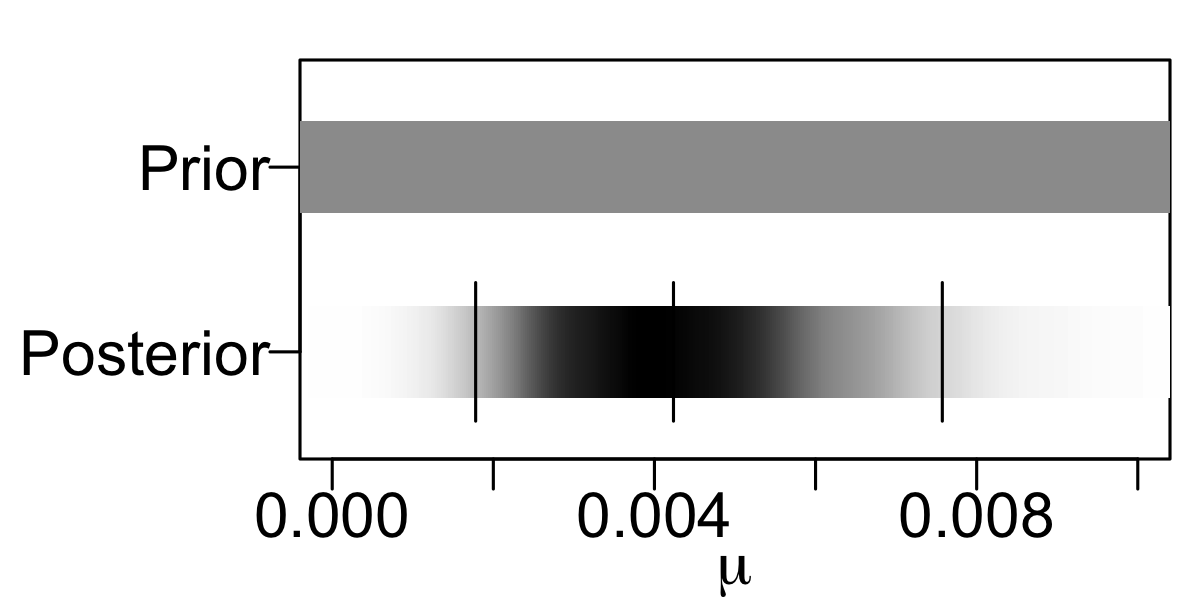
\includegraphics[width=\textwidth]{figures/figure_2a.png}
		\caption{}
		\label{fig:mu_density}
	\end{subfigure}
	\hfill
	\begin{subfigure}[b]{0.3\textwidth}
		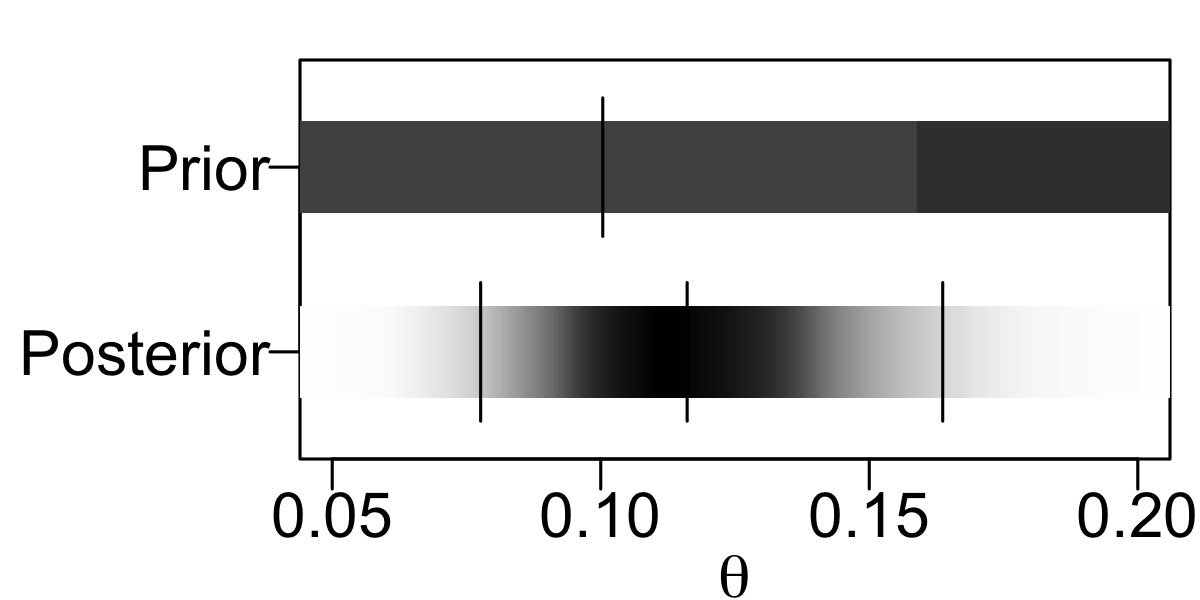
\includegraphics[width=\textwidth]{figures/figure_2b.png}
		\caption{}
		\label{fig:theta_density}
	\end{subfigure}
	\hfill
	\begin{subfigure}[b]{0.3\textwidth}
		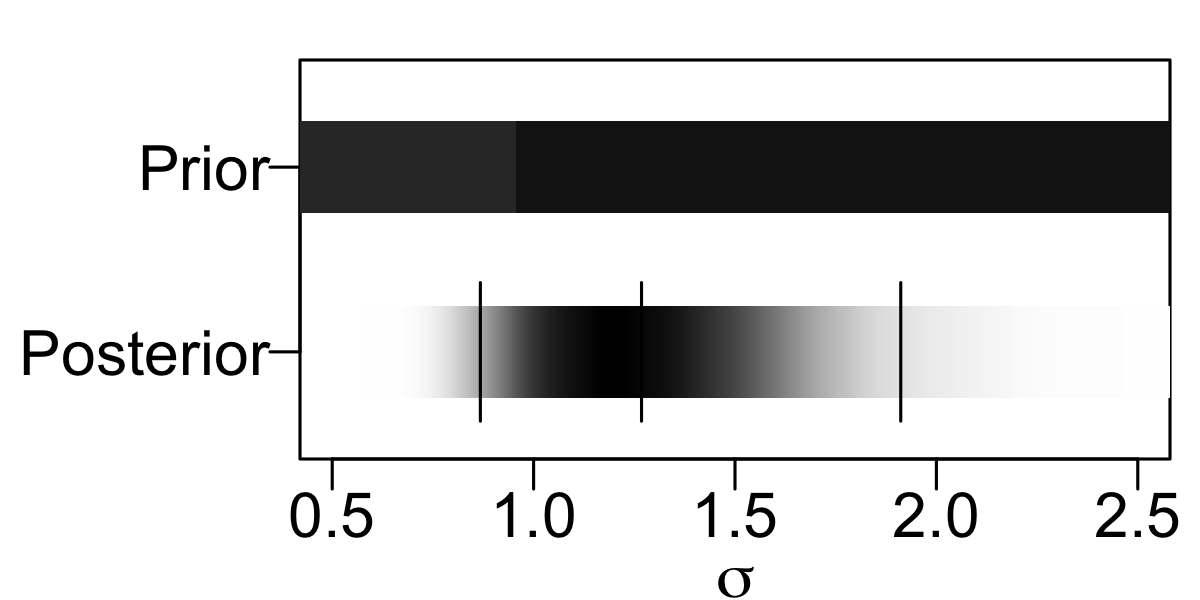
\includegraphics[width=\textwidth]{figures/figure_2c.png}
		\caption{}
		\label{fig:sigma_density}
	\end{subfigure} 
	\medskip
		\begin{subfigure}[b]{0.3\textwidth}
		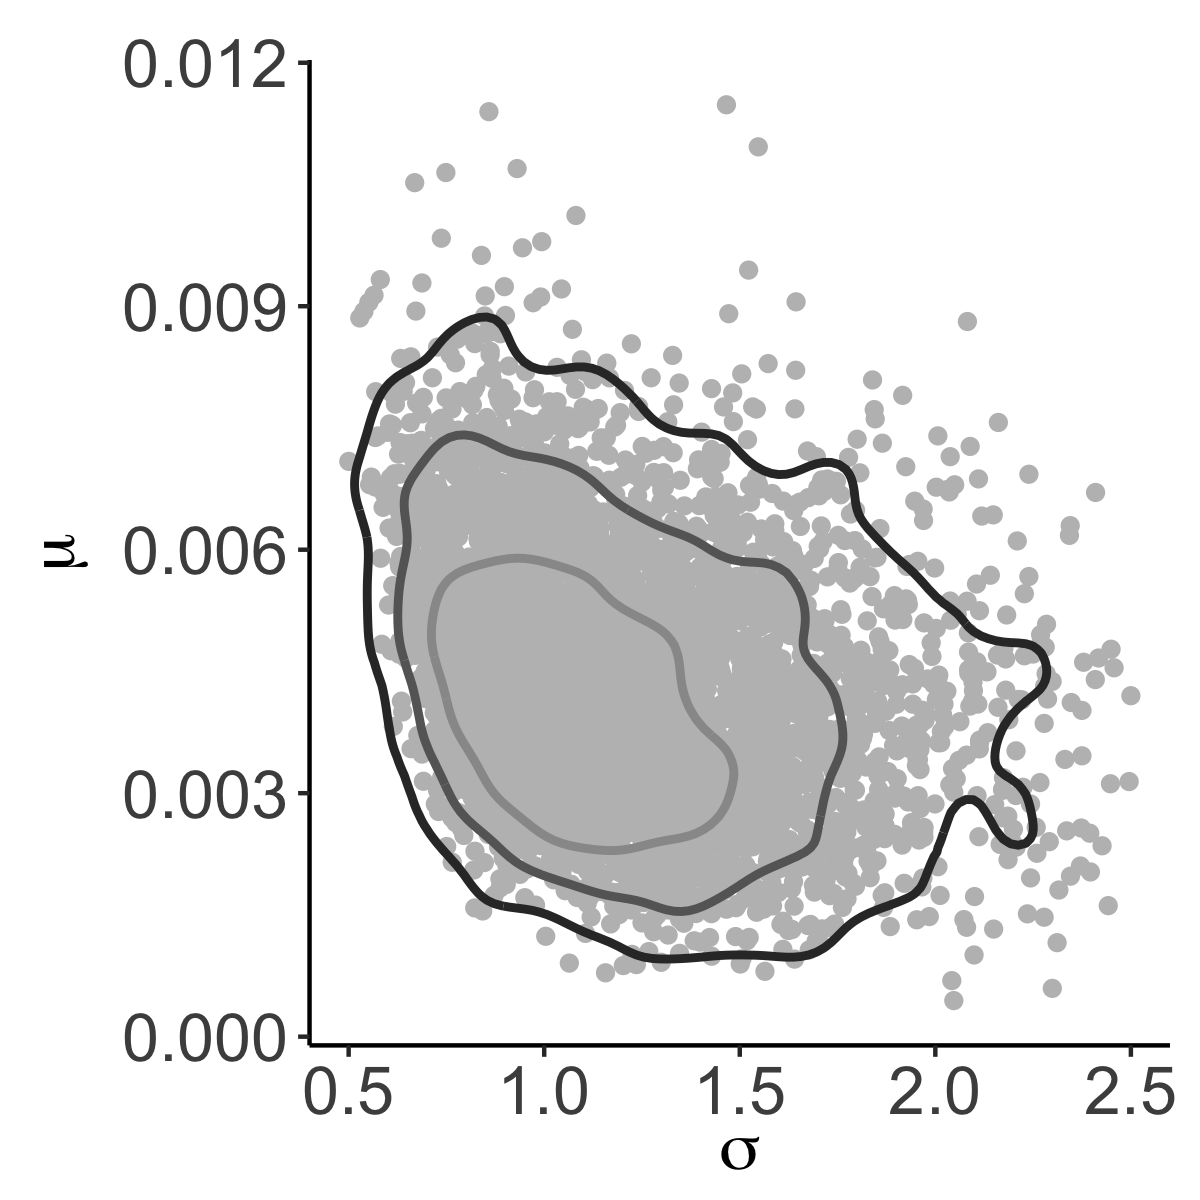
\includegraphics[width=\textwidth]{figures/figure_2d.png}
		\caption{}
		\label{fig:muSigma}
	\end{subfigure}
	\hfill
	\begin{subfigure}[b]{0.3\textwidth}
		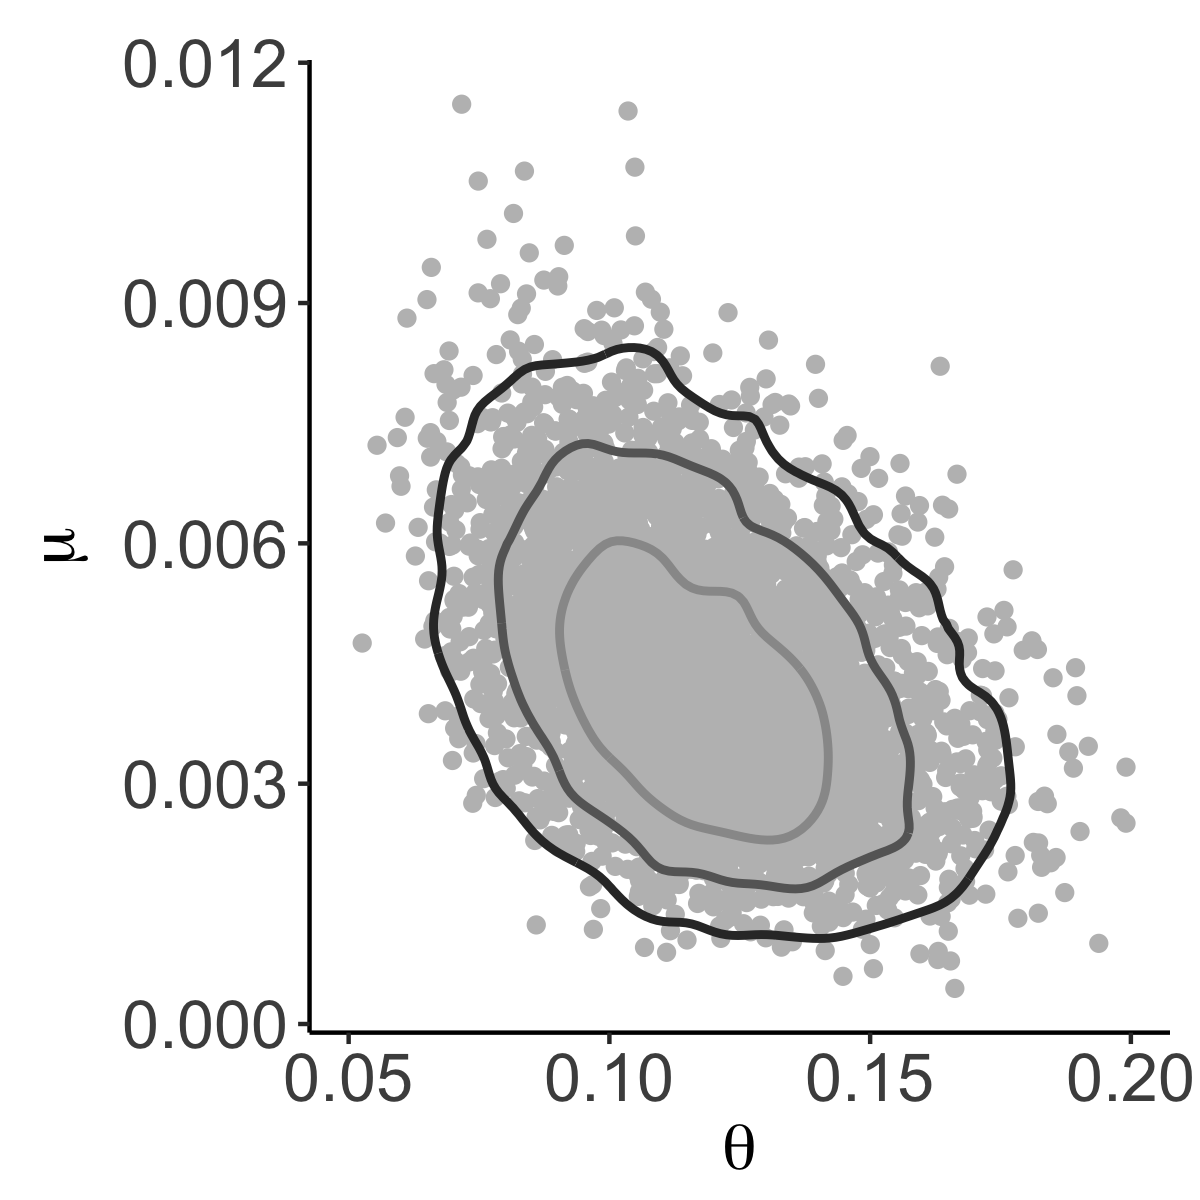
\includegraphics[width=\textwidth]{figures/figure_2e.png}
		\caption{}
		\label{fig:muTheta}
	\end{subfigure}
	\hfill
	\begin{subfigure}[b]{0.3\textwidth}
		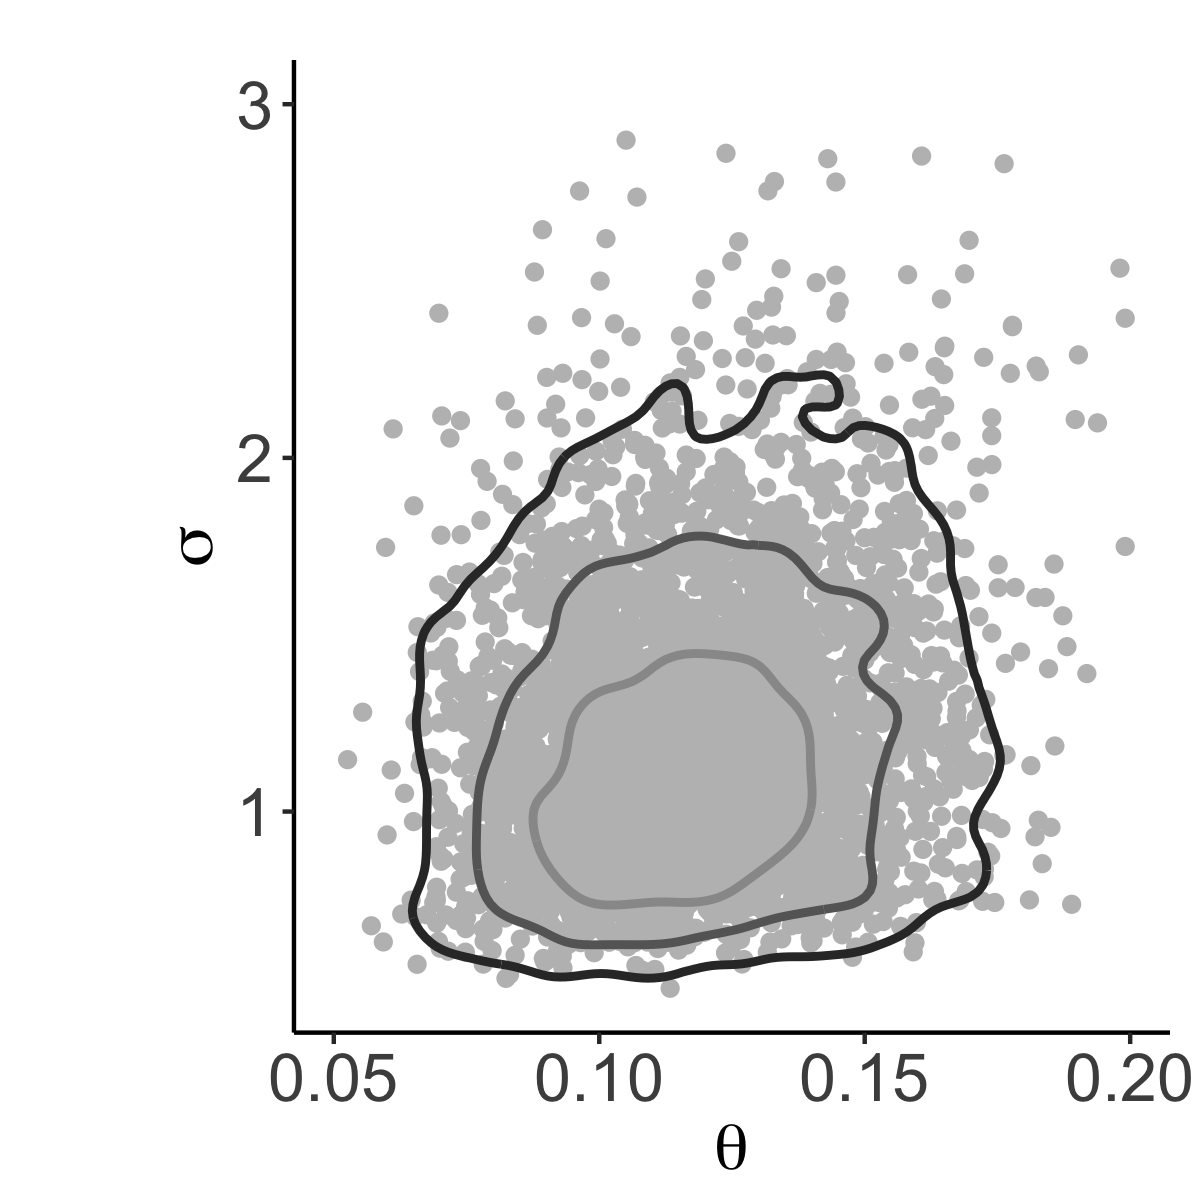
\includegraphics[width=\textwidth]{figures/figure_2f.png}
		\caption{}
		\label{fig:sigmaTheta}
	\end{subfigure} 
	\caption{(\subref{fig:mu_density}) - (\subref{fig:sigma_density}) shows the parameter densities;  (\subref{fig:muSigma}) - (\subref{fig:sigmaTheta}) shows pairwise posterior samples }
	\label{fig:muSigmaThetaDensities}
\end{figure} 



\begin{figure}[H]
	\centering
	\begin{subfigure}[b]{0.49\textwidth}
		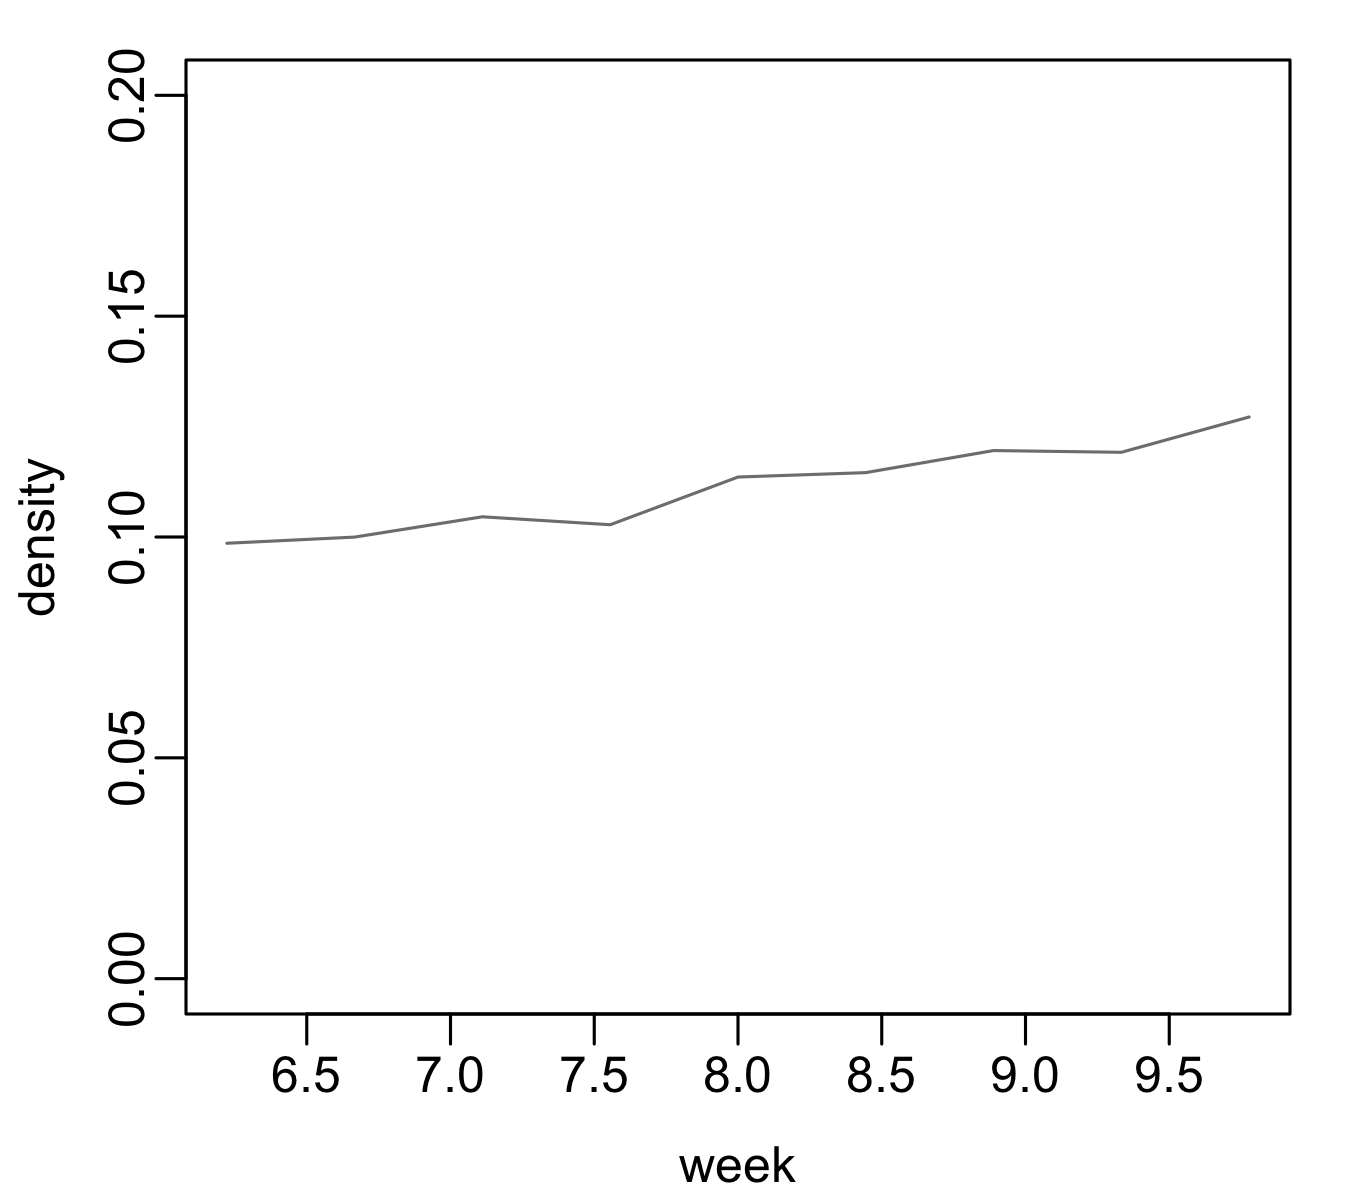
\includegraphics[width=\textwidth]{figures/figure_3a.png}
		\caption{}
		\label{fig:first_infections}
	\end{subfigure}
	\hfill
	\begin{subfigure}[b]{0.49\textwidth}
		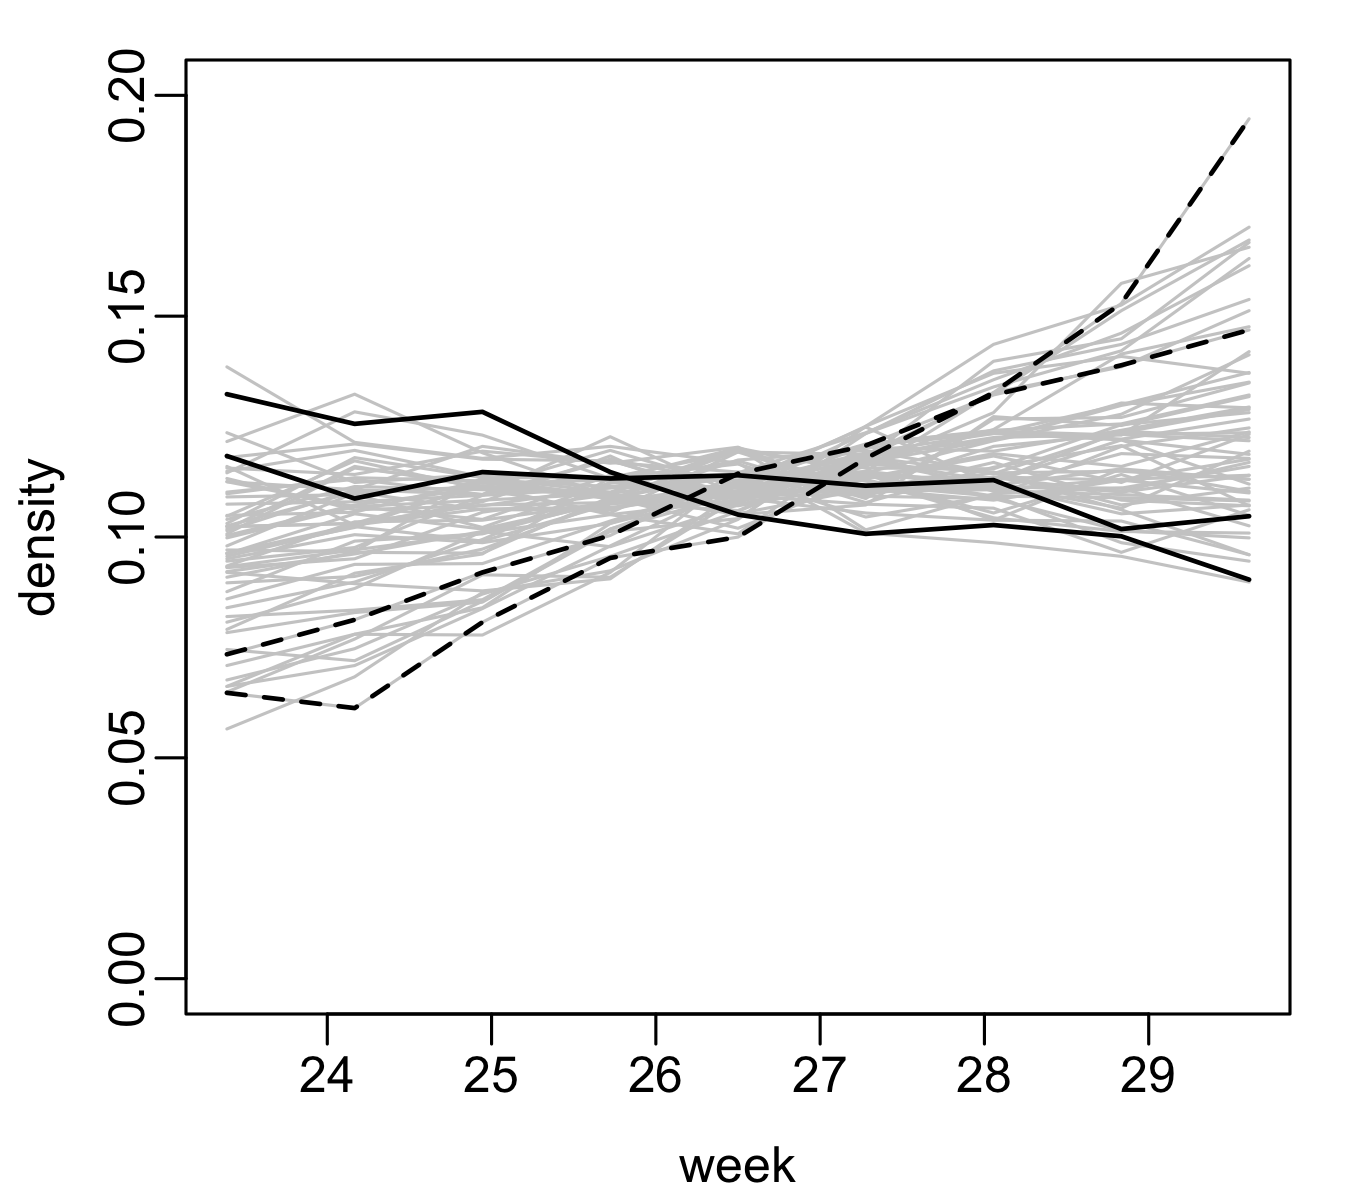
\includegraphics[width=\textwidth]{figures/figure_3b.png}
		\caption{}
		\label{fig:last_infections}
	\end{subfigure}
	\caption{(\subref{fig:first_infections}) tbd; (\subref{fig:last_infections}) tbd }
	\label{fig:data_plot}
\end{figure} 



\begin{figure}[H]
	\centering
	\begin{subfigure}[b]{0.49\textwidth}
		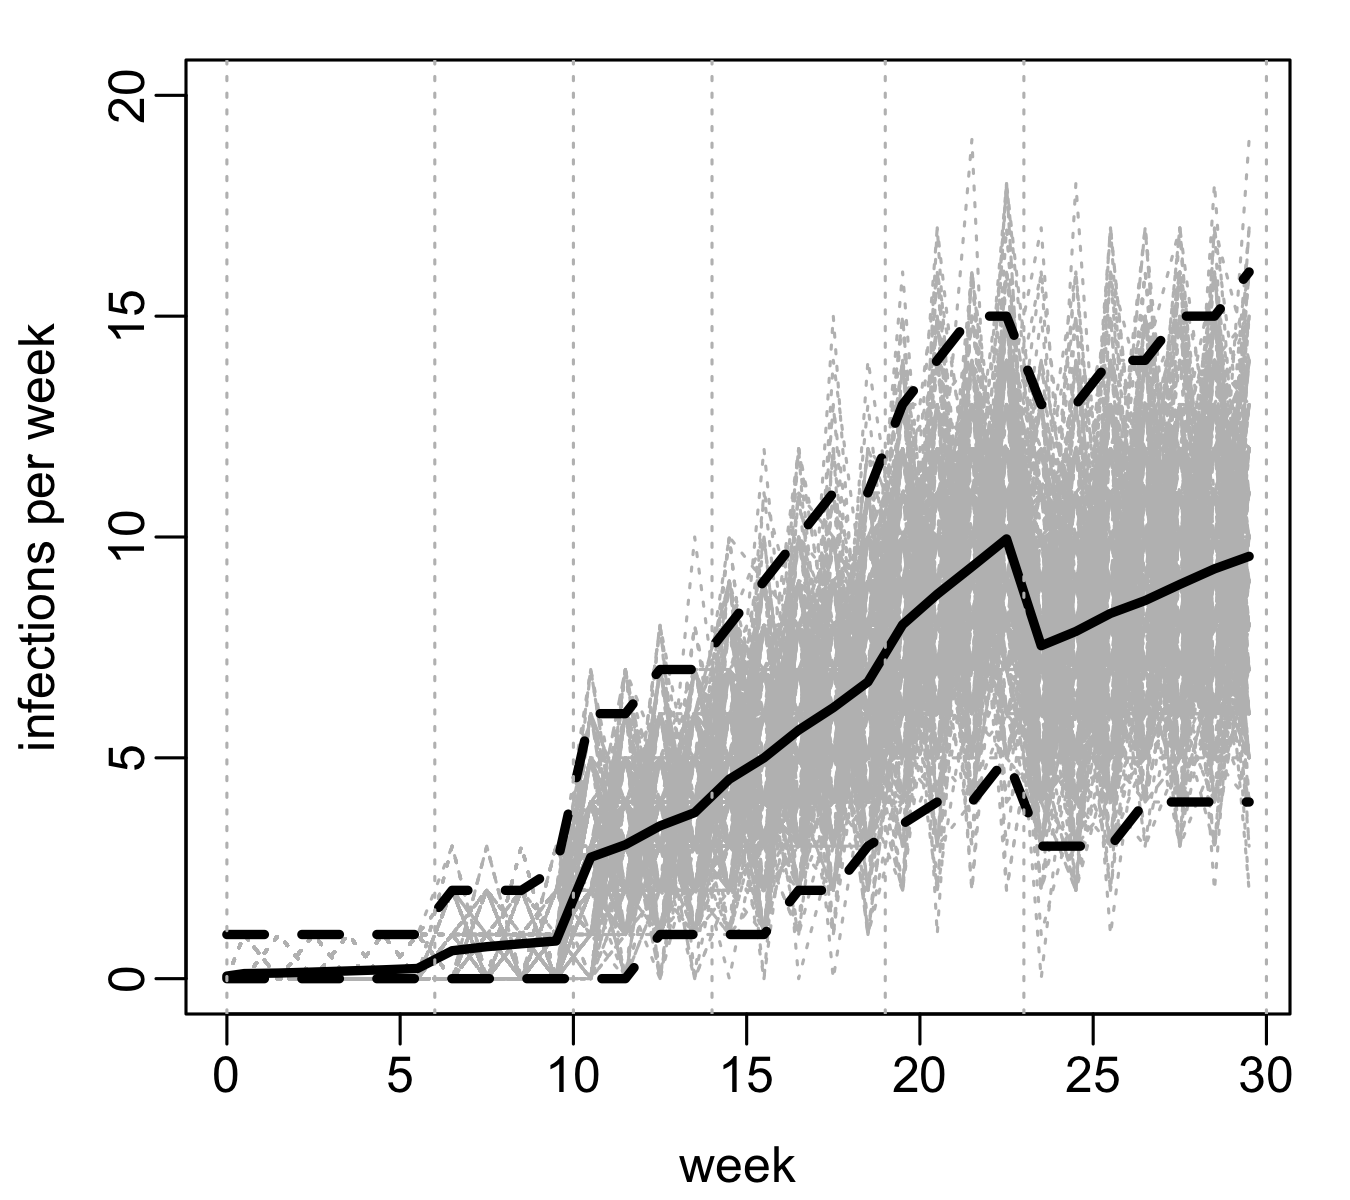
\includegraphics[width=\textwidth]{figures/figure_4a.png}
		\caption{}
		\label{fig:cond_infections}
	\end{subfigure}
	\hfill
	\begin{subfigure}[b]{0.49\textwidth}
		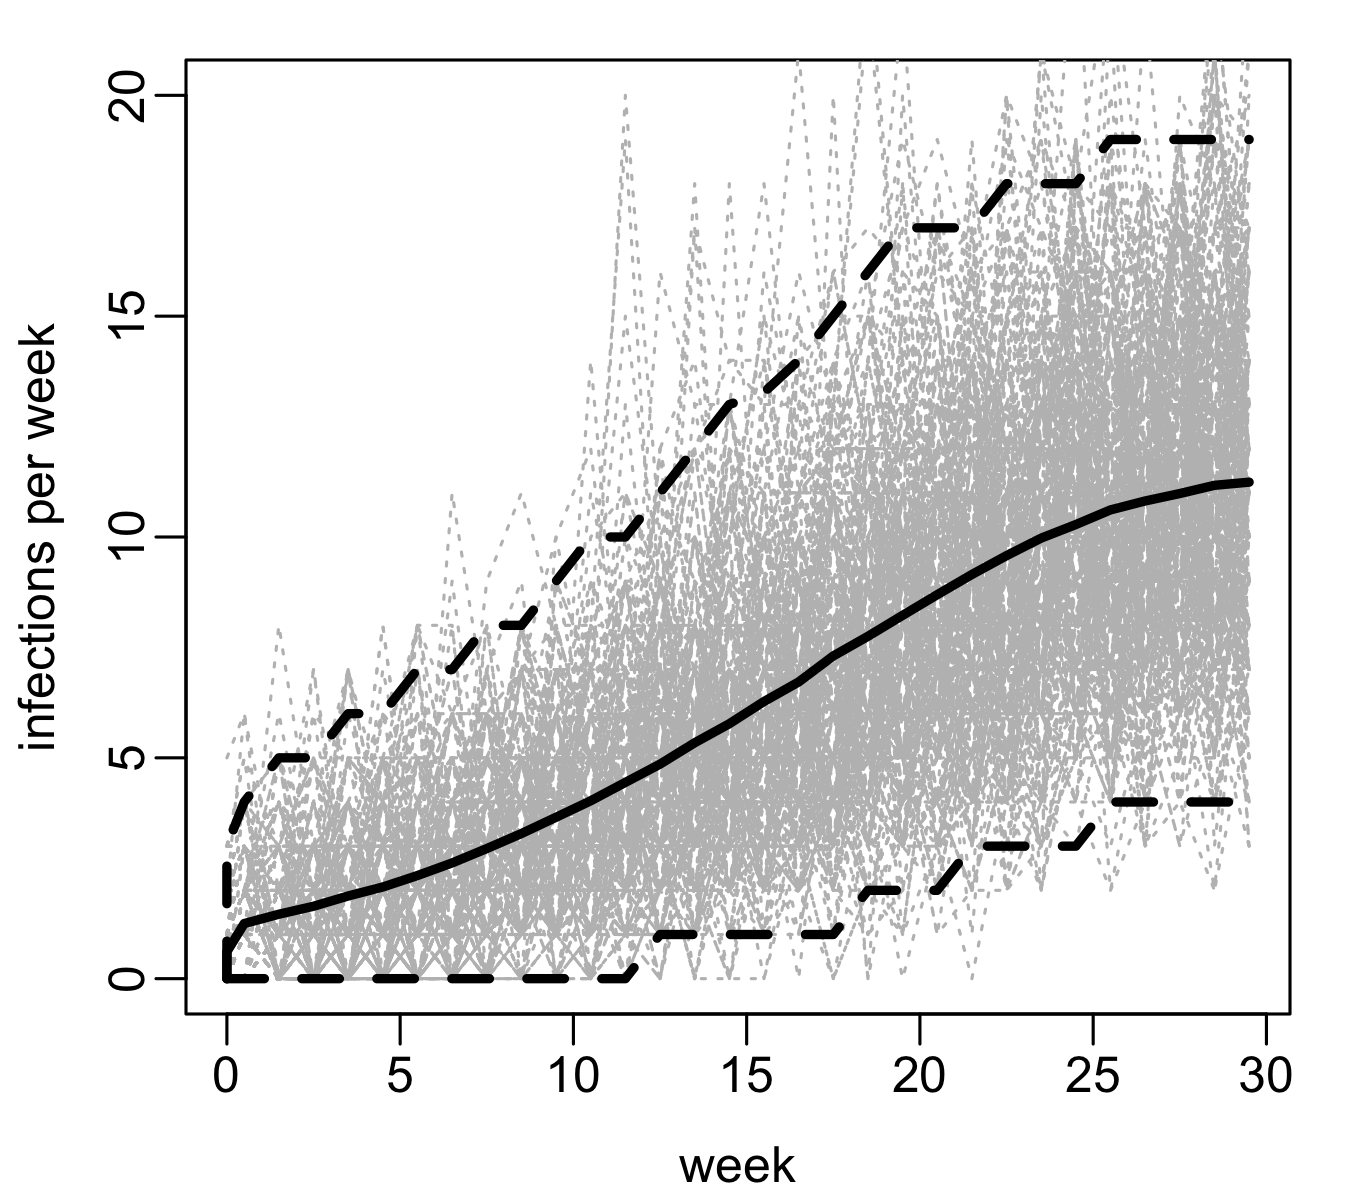
\includegraphics[width=\textwidth]{figures/figure_4b.png}
		\caption{}
		\label{fig:sim_infection}
	\end{subfigure}
	\caption{(\subref{fig:cond_infections}) tbd; (\subref{fig:sim_infection}) tbd }
	\label{fig:data_plot}
\end{figure} 


\begin{figure}[H]
	\centering
	\begin{subfigure}[b]{0.49\textwidth}
		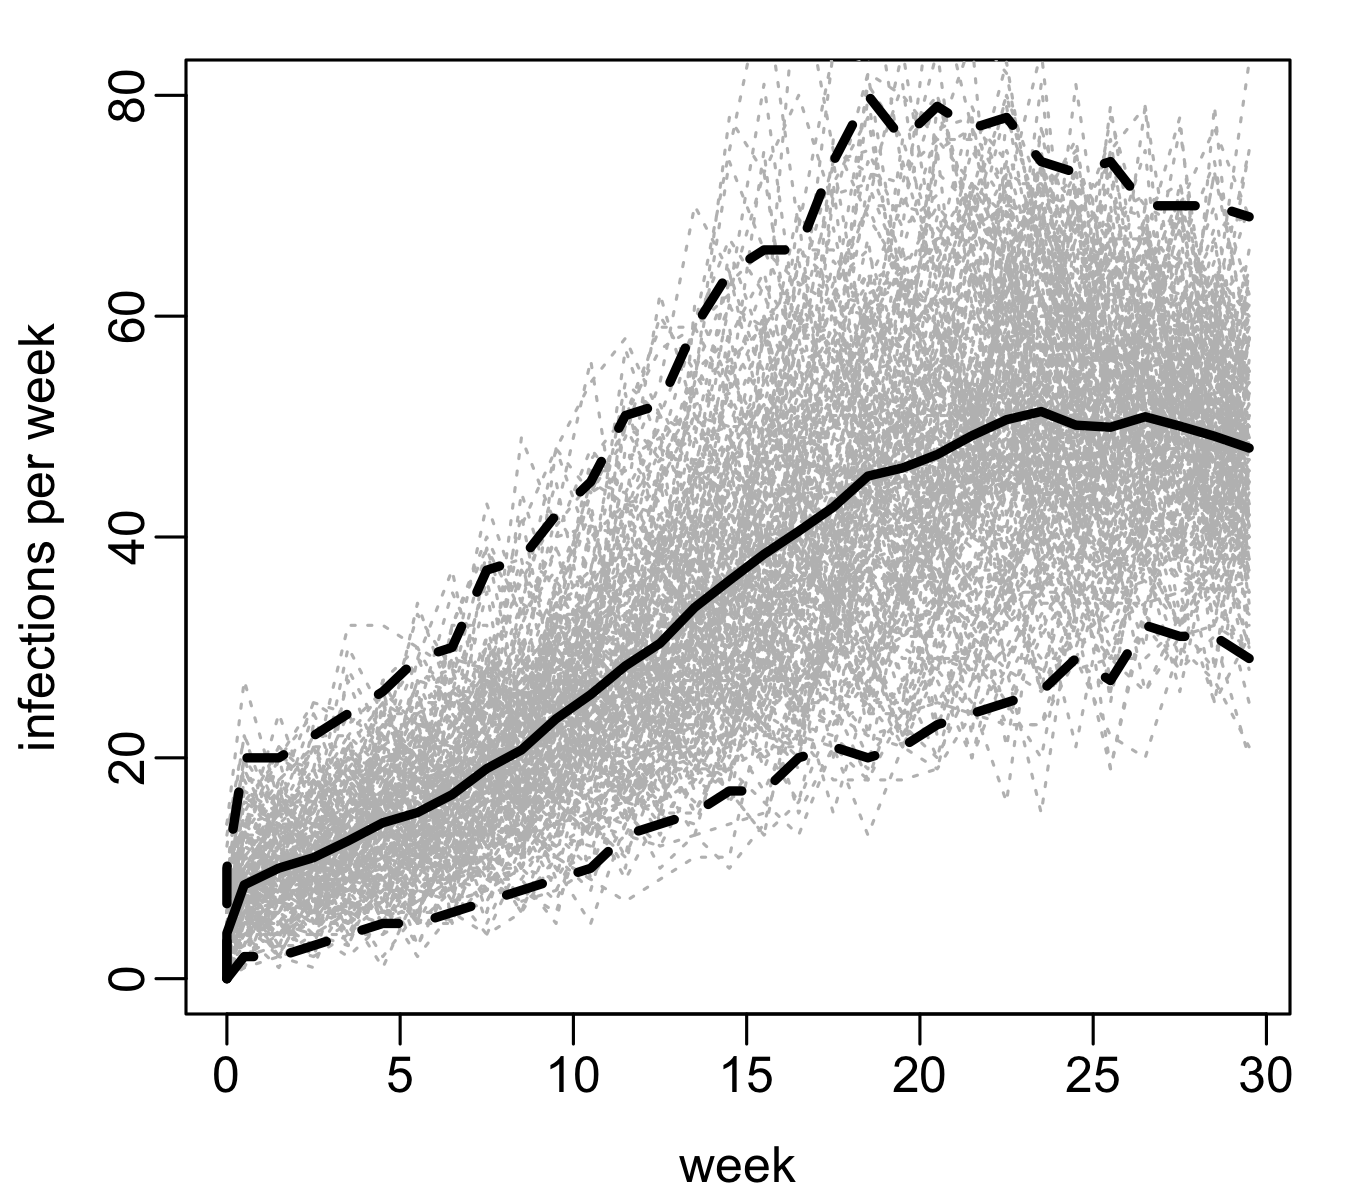
\includegraphics[width=\textwidth]{figures/figure_4b_all_plants.png}
		\caption{}
		\label{fig:all_infections}
	\end{subfigure}
	\hfill
	\begin{subfigure}[b]{0.49\textwidth}
		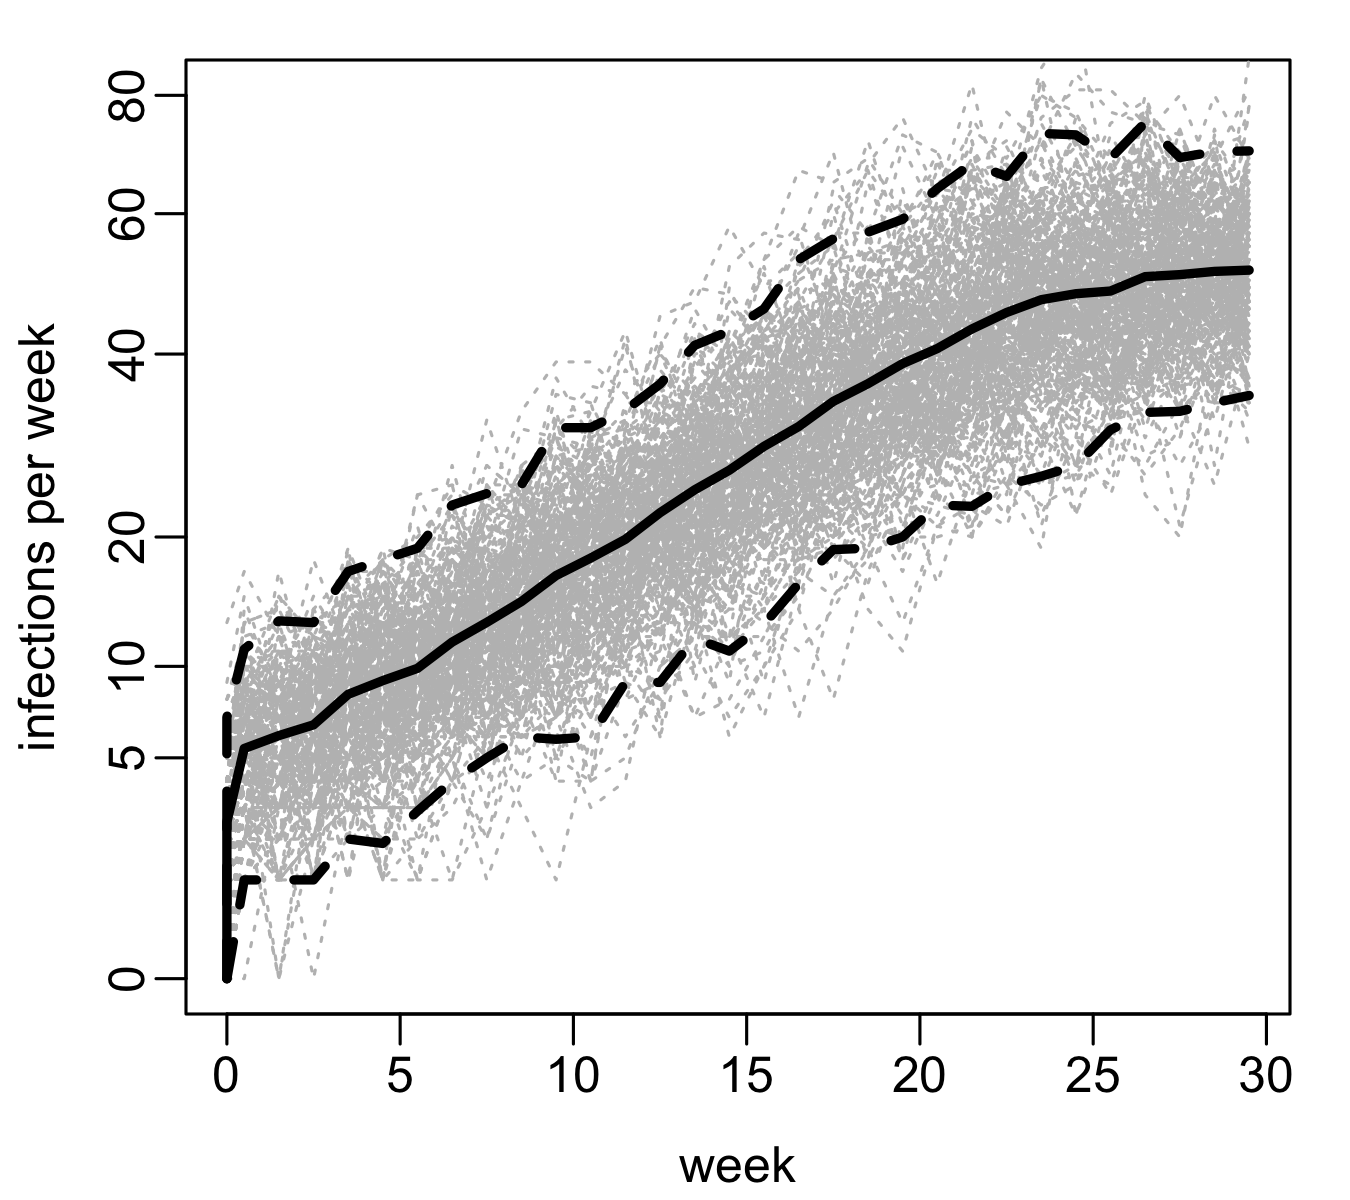
\includegraphics[width=\textwidth]{figures/figure_4b_all_plants_root.png}
		\caption{}
		\label{fig:root_all_infections}
	\end{subfigure}
	\caption{(\subref{fig:all_infections}) tbd; (\subref{fig:root_all_infections}) tbd }
	\label{fig:data_plot}
\end{figure} 


\begin{figure}[H]
	\centering
	\begin{subfigure}[b]{0.24\textwidth}
		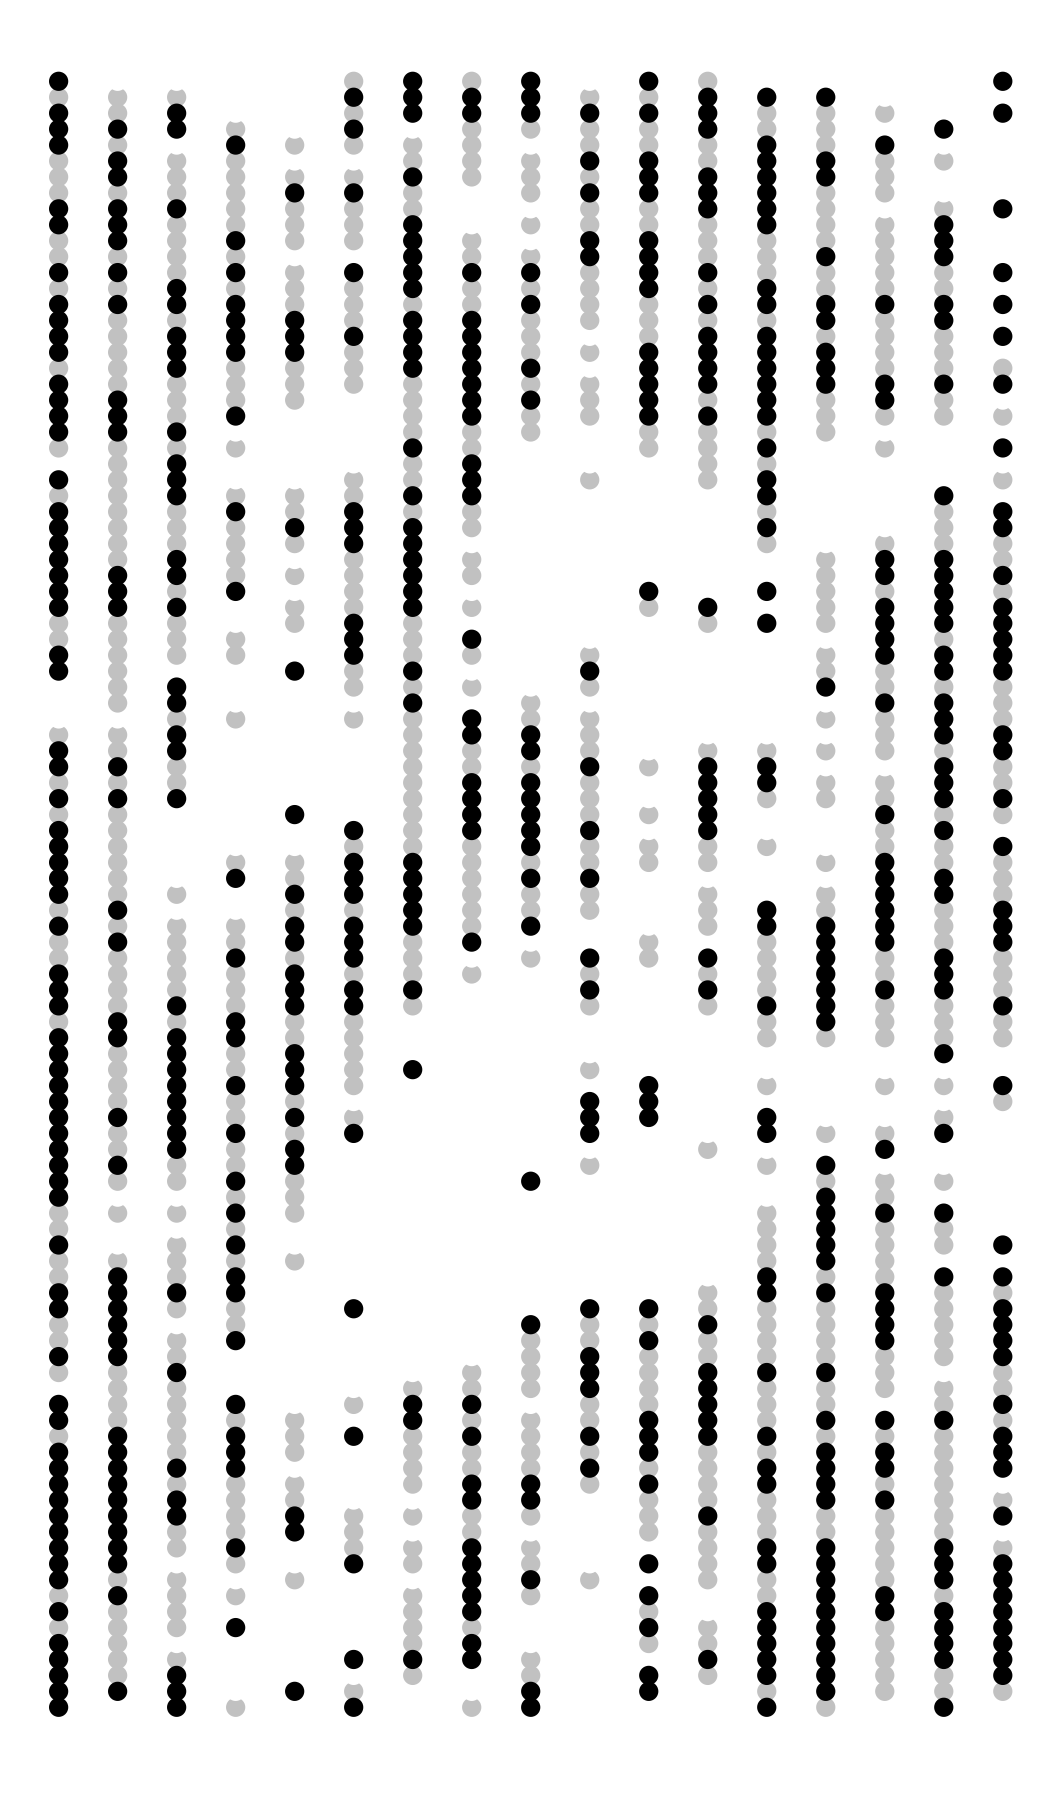
\includegraphics[width=\textwidth]{figures/figure_5a.png}
		\caption{}
		\label{fig:week_35}
	\end{subfigure}
	\hfill
	\begin{subfigure}[b]{0.24\textwidth}
		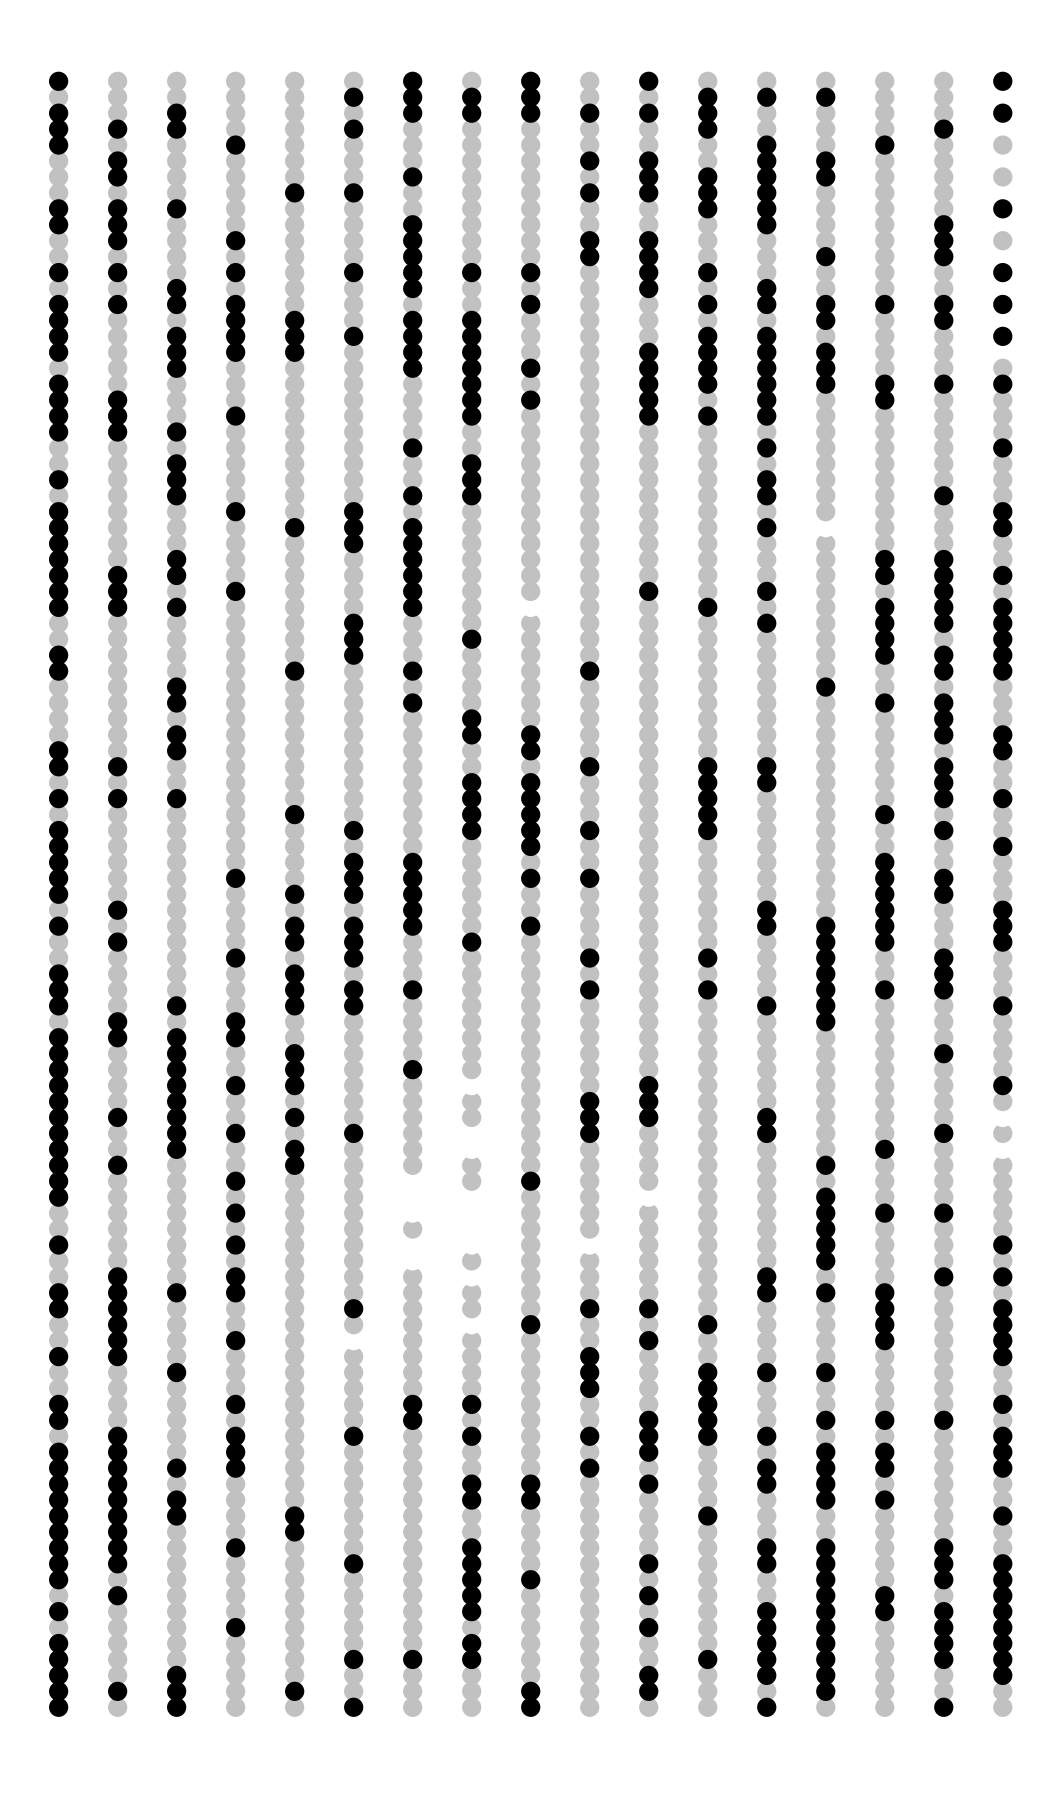
\includegraphics[width=\textwidth]{figures/figure_5b.png}
		\caption{}
		\label{fig:week_40}
	\end{subfigure}
	\hfill
	\begin{subfigure}[b]{0.24\textwidth}
		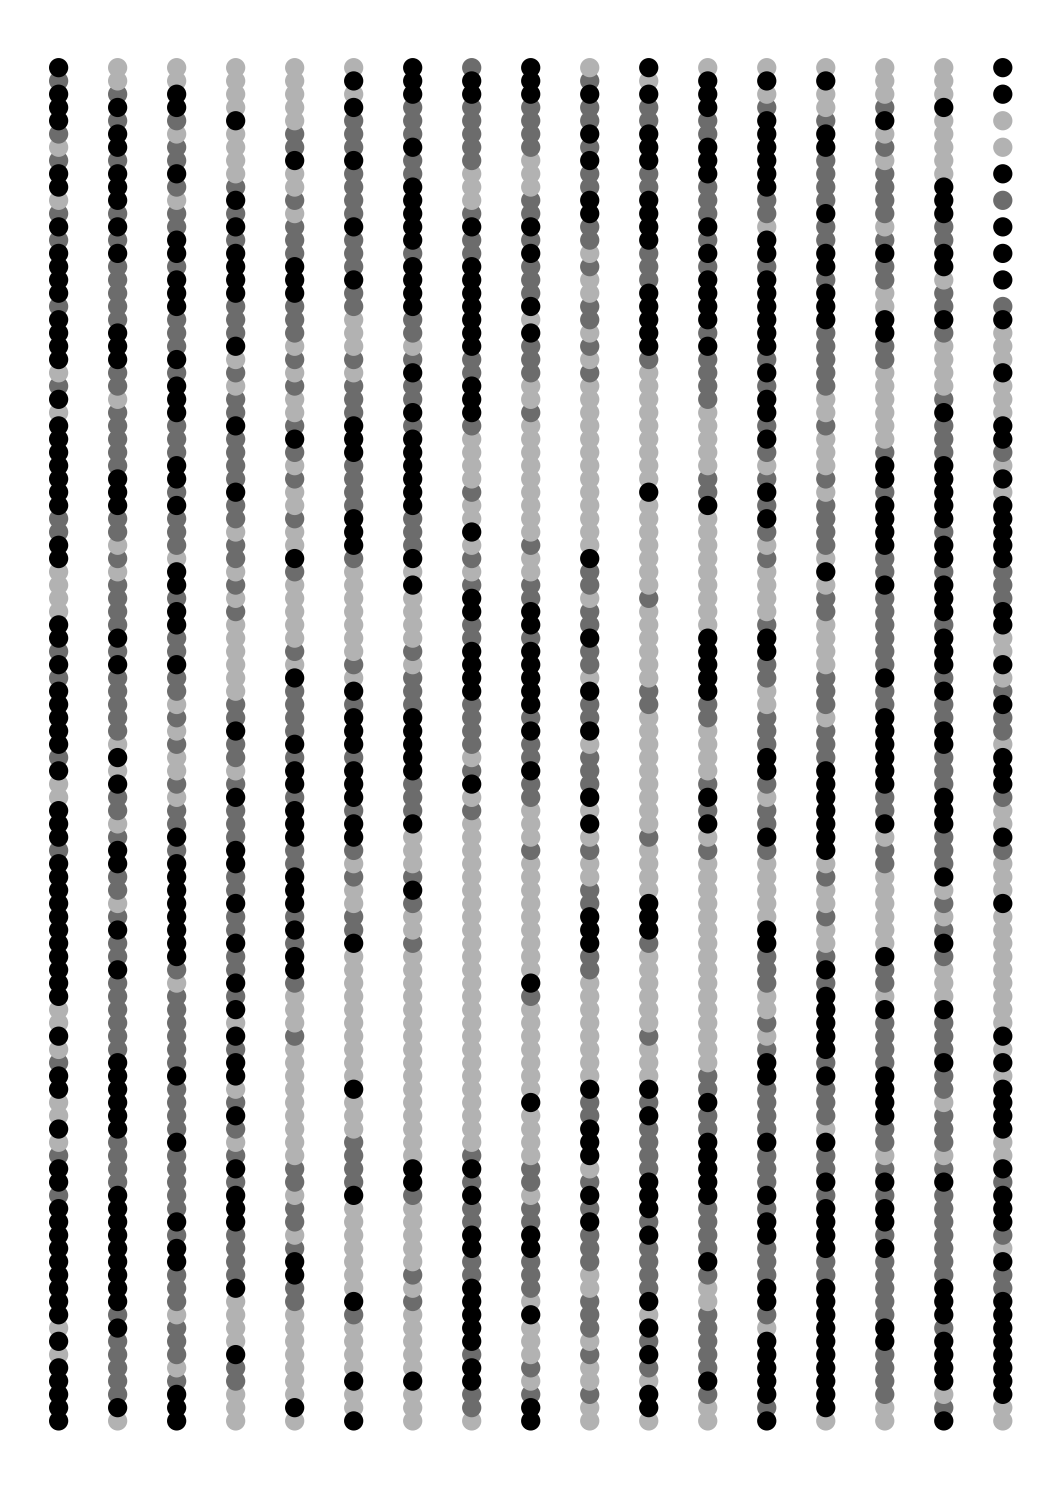
\includegraphics[width=\textwidth]{figures/figure_5c.png}
		\caption{}
		\label{fig:week_50}
	\end{subfigure}
	\hfill
	\begin{subfigure}[b]{0.24\textwidth}
		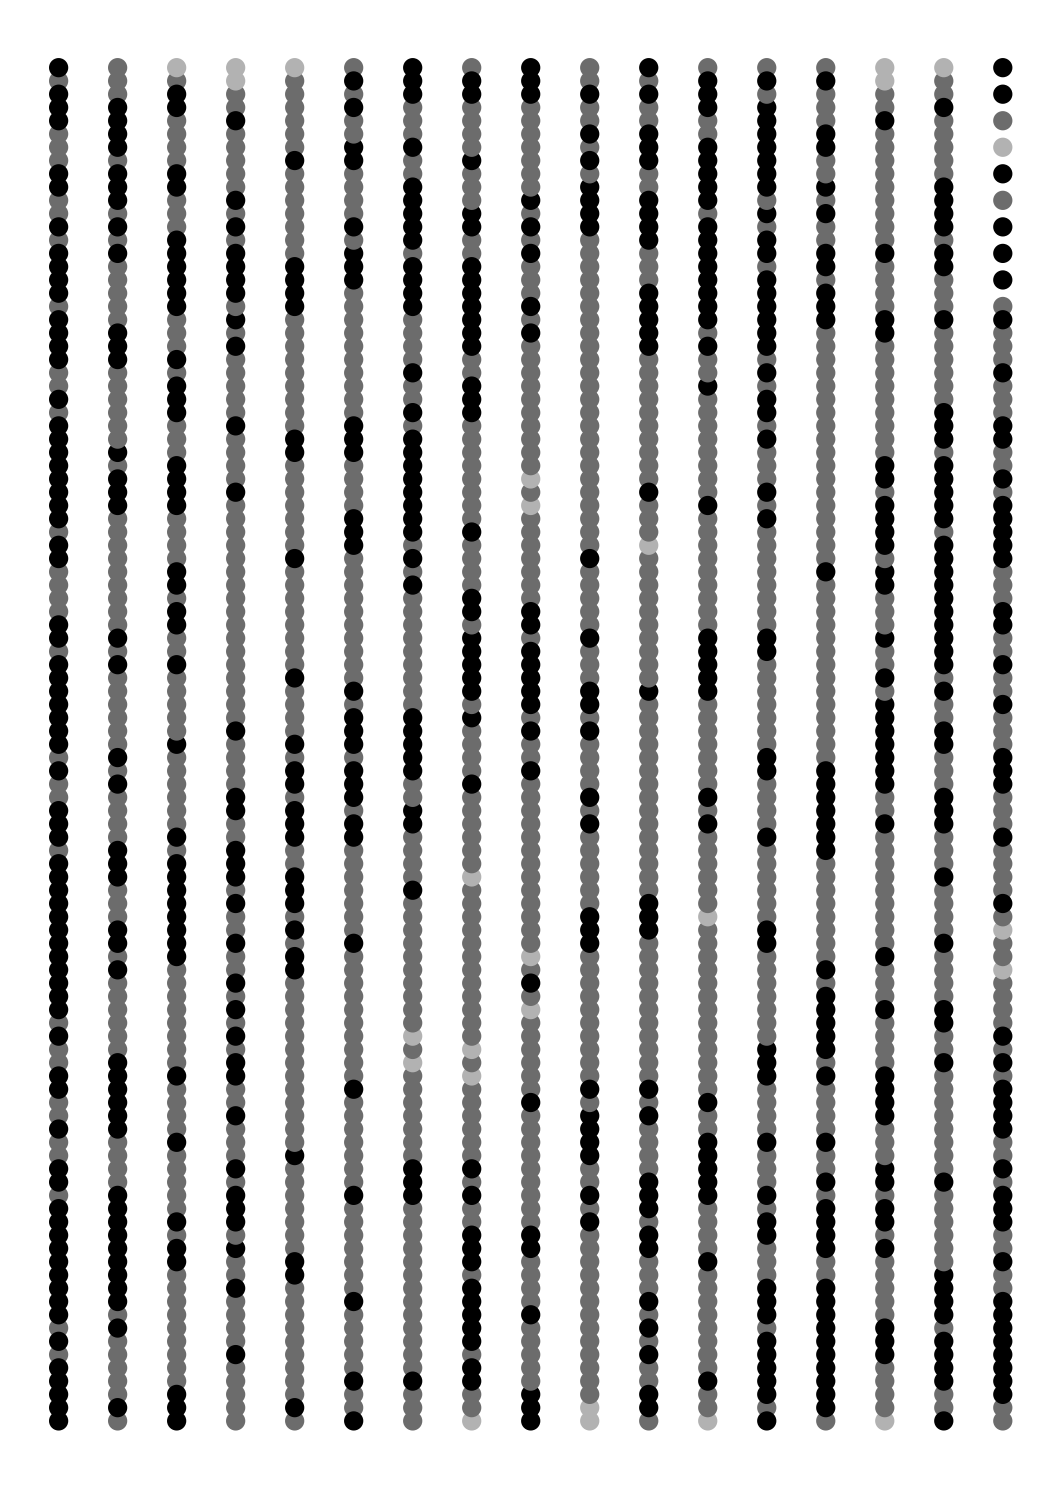
\includegraphics[width=\textwidth]{figures/figure_5d.png}
		\caption{}
		\label{fig:week_60}
	\end{subfigure}
	\caption{(\subref{fig:week_35}) tbd; (\subref{fig:week_60}) tbd }
	\label{fig:data_plot}
\end{figure} 

While \citet{Brown} presents several variations of the basic and parallel Metropolis algorithms that improve performance, the authors ultimately determined that the statistical model specified was incapable of capturing the underlying complexities of the plantation data. 
After deriving the parameters for the prior on $\mu$ and simulating epidemics from a subsample of the data, it became clear that the findings reported in \citet{Brown} were based on a flawed Metropolis algorithm implementation. 
Coding errors were replicated across all implementations and ultimately led the authors to possibly unfounded inference. 

Coding the MCMC algorithm as suggested in \citet{Brown} led to run times many orders of magnitude slower than the times reported. 
Running times were prohibitively slow even after taking a 10\% sample of the full data set. 
While this is to be expected for the R prototype, Julia benchmarks against the C programming language indicate that the performance difference cannot be fully explained by the choice of programming language. 
Each method was coded according to standard software engineering best practices, including modular programming and test-driven development approach.  

Simulating new epidemics from the posterior parameters conditioned on the infection intervals and from the posterior parameters alone led \citet{Brown} to the results in figure \ref{fig:post_sim_plot}. 
Comparing the published simulated epidemics based on posterior samples for the number of new infections per week conditioned on the six observations with simulated epidemics based on the posterior parameters without reference to the data shows that the unconditional simulated outbreaks begin much faster than what the data supports. 
This result is completely determined by the endemic infection rate, $\mu$. 
Now, time to the first infection is distributed as an exponential random variable with rate $\mu$. 
If $\mu$ were somehow overestimated, then the time to the first infection would drop substantially.
In this case, the mismatch between the conditional and unconditional simulations in figure \ref{fig:post_sim_plot} are due to an error in the Metropolis sampler. 
Instead of using weakly informative prior $\mu \sim \Gamma(0.7, \text{rate}=0.004)$ with mean 175 and variance $\frac{0.7}{0.004^2}=43,750$, \citep{Brown} specified $\mu \sim \Gamma(0.7, \text{scale}=0.004)$ with mean 0.0028 and variance $1.12\times10^{-5}$. 
As a result, it is clear from figure \ref{fig:prior_mu_plot} that the posterior samples for $\mu$ only reflects the influence of the prior. 
After reviewing the authors' source code, it was confirmed that the authors did in fact use the scale parameterization for all gamma priors in the sampler. 
As a result, $\sigma$ is the only prior properly encoded. 

\begin{table}[ht]
\centering
\begin{tabular}{r|rrrrr}
  Algorithm & \multicolumn{5}{c}{Times for Updating the Following Parameters} \\
 \hline
 & $\theta$ & $\mu$ & $\tau$ & $\sigma$ & Total \\ 
  \hline
  Basic & 28.15 & 14.27 & 160.92 & 28.99 & 232.33 \\ 
  Parallel & 25.08 & 12.57 & 29.99 & 25.17 & 92.81 \\ 
  Truncated & 1.07 & 1.07 & 1.76 & 1.13 & 5.03 \\ 
  \hline
\end{tabular}
\caption{tbd...}
\end{table}


\section{Discussion}

\newpage
\bibliography{prelim_references}

\newpage
\appendix
\section{Metropolis Algorithm Diagnostic Plots}
\label{metropolis_plots}

\begin{figure}[H]
	\centering
	\begin{subfigure}[b]{0.49\textwidth}
		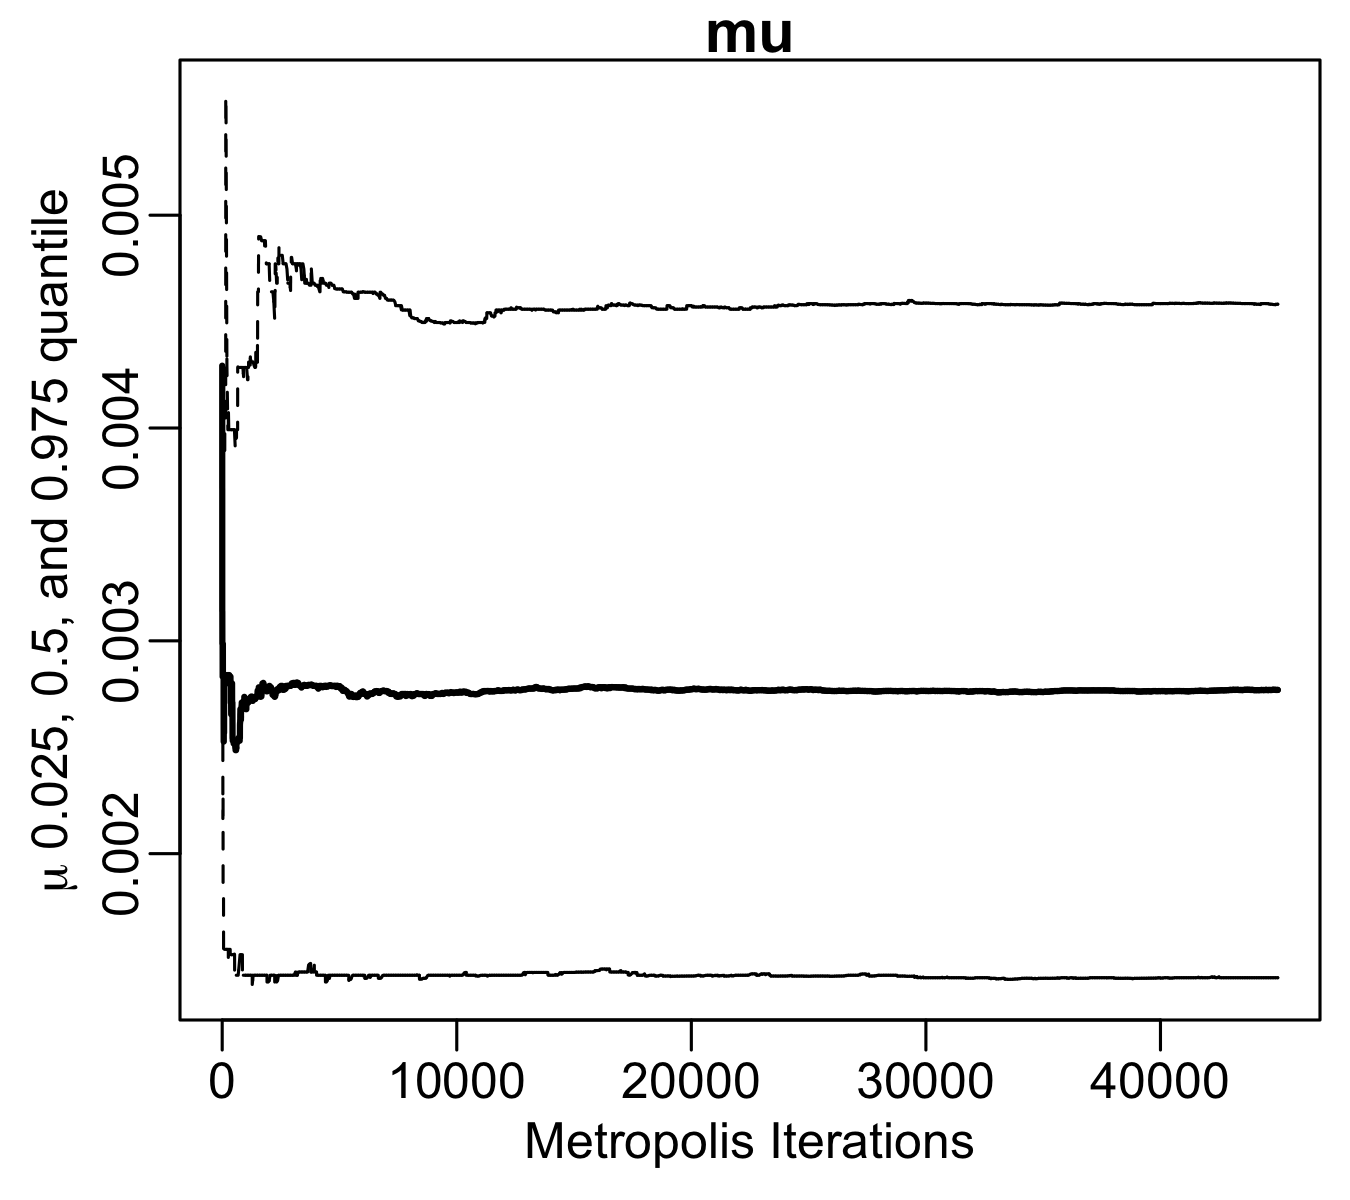
\includegraphics[width=\textwidth]{figures/mcmc_cum_quant_plot_mu.png}
		\caption{}
		\label{fig:quant_mu}
	\end{subfigure}
	\hfill
	\begin{subfigure}[b]{0.49\textwidth}
		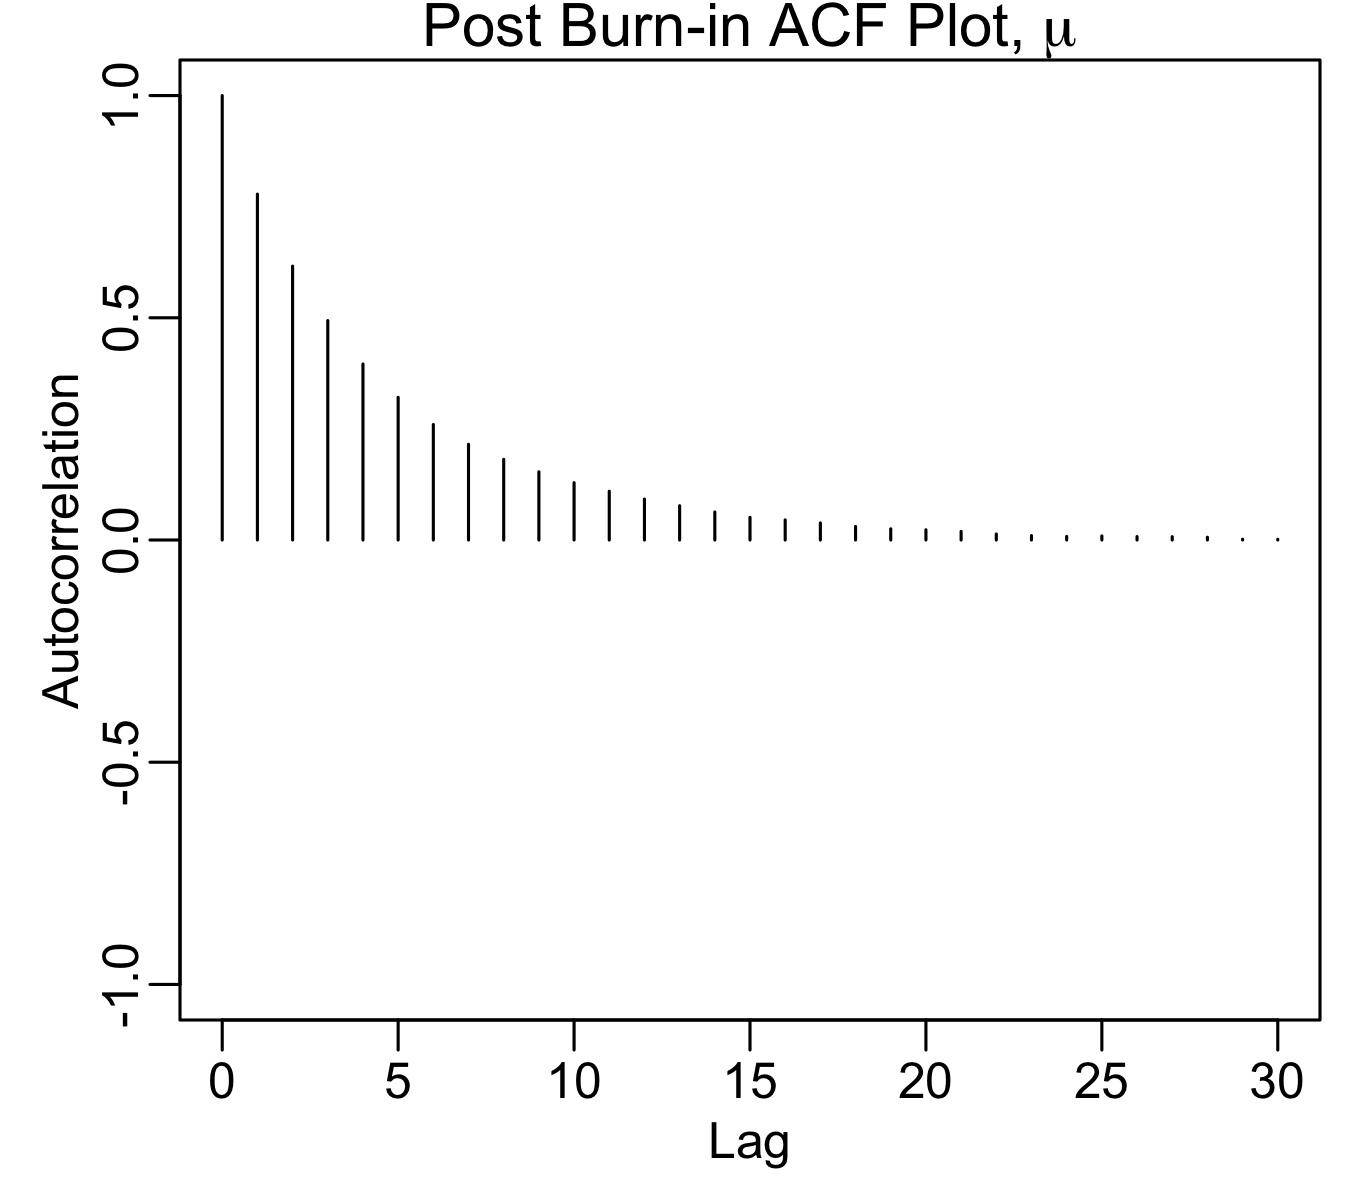
\includegraphics[width=\textwidth]{figures/mcmc_acf_plot_mu.png}
		\caption{}
		\label{fig:acf_mu}
	\end{subfigure}
	\caption{(\subref{fig:quant_mu}) tbd; (\subref{fig:acf_mu}) tbd }
	\label{fig:data_plot}
\end{figure} 

\begin{figure}[H]
	\centering
	\begin{subfigure}[b]{0.49\textwidth}
		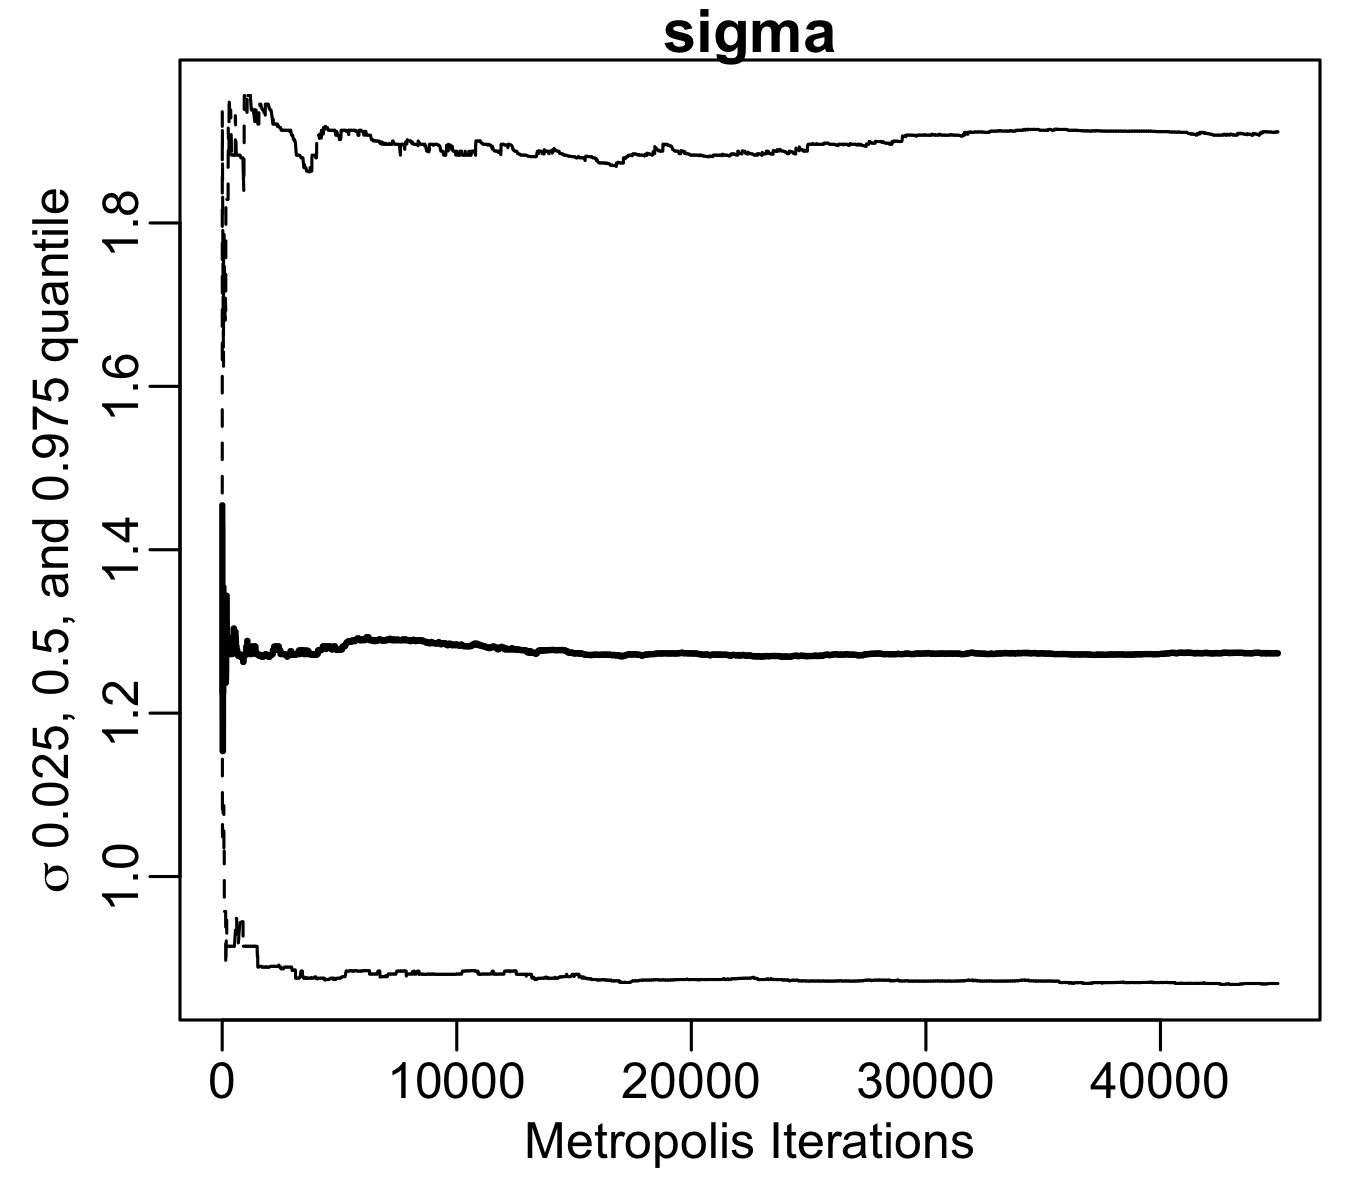
\includegraphics[width=\textwidth]{figures/mcmc_cum_quant_plot_sigma.png}
		\caption{}
		\label{fig:quant_sigma}
	\end{subfigure}
	\hfill
	\begin{subfigure}[b]{0.49\textwidth}
		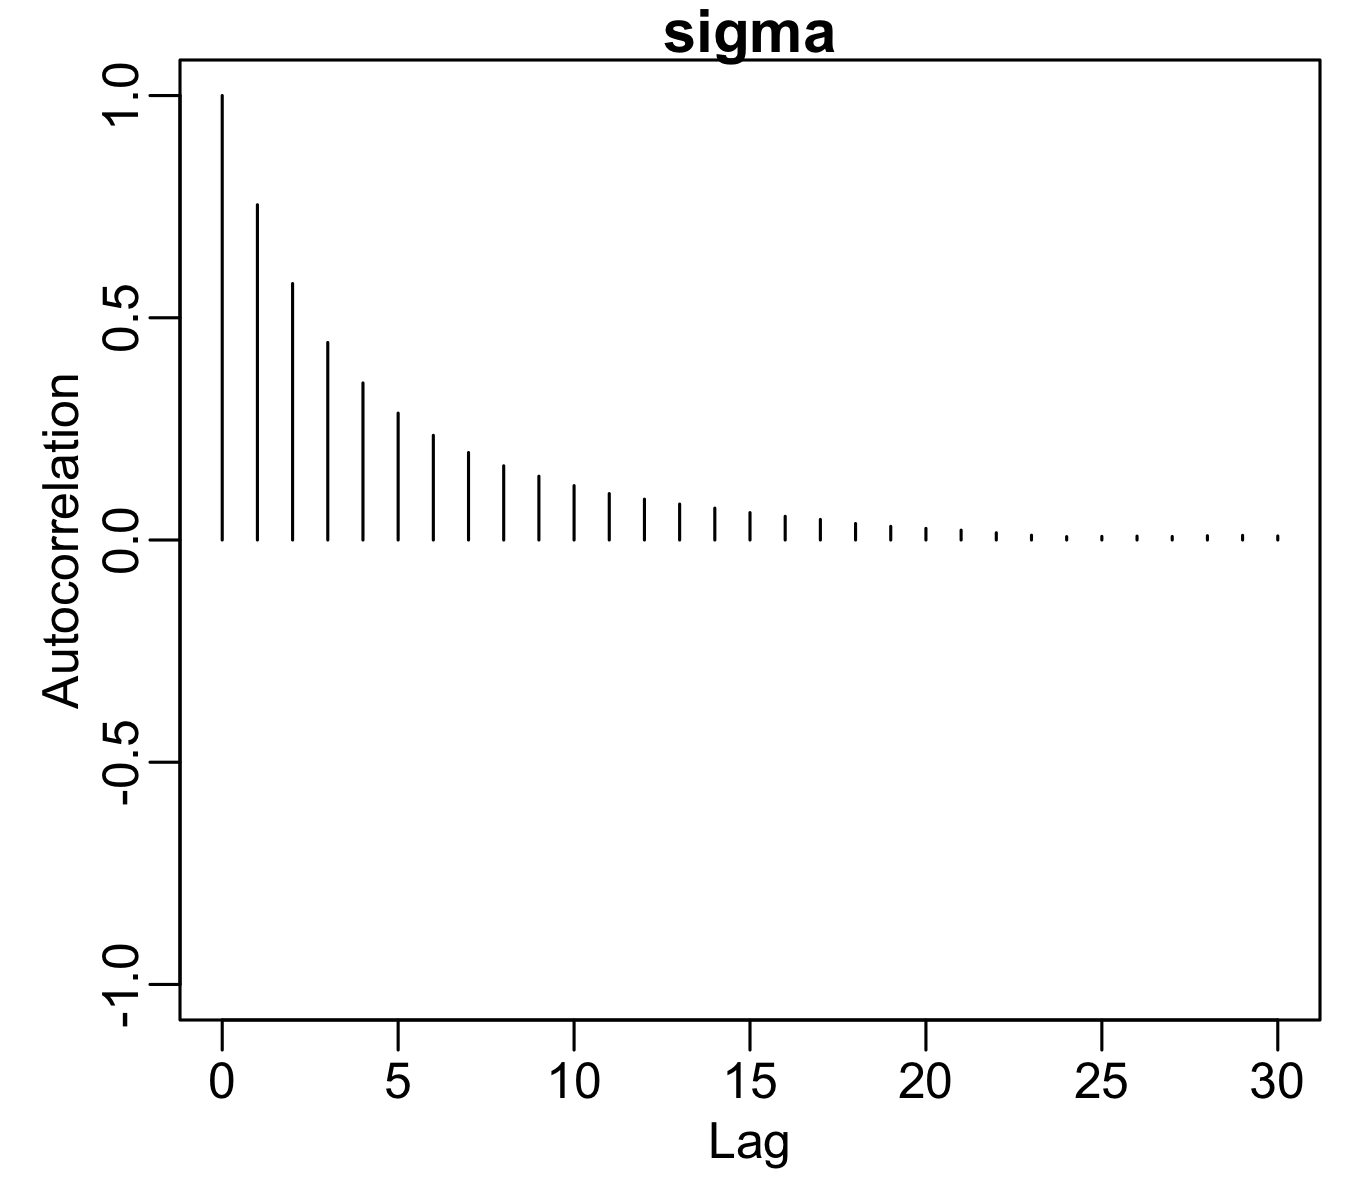
\includegraphics[width=\textwidth]{figures/mcmc_acf_plot_sigma.png}
		\caption{}
		\label{fig:acf_sigma}
	\end{subfigure}
	\caption{(\subref{fig:quant_sigma}) tbd; (\subref{fig:acf_sigma}) tbd }
	\label{fig:data_plot}
\end{figure} 

\begin{figure}[H]
	\centering
	\begin{subfigure}[b]{0.49\textwidth}
		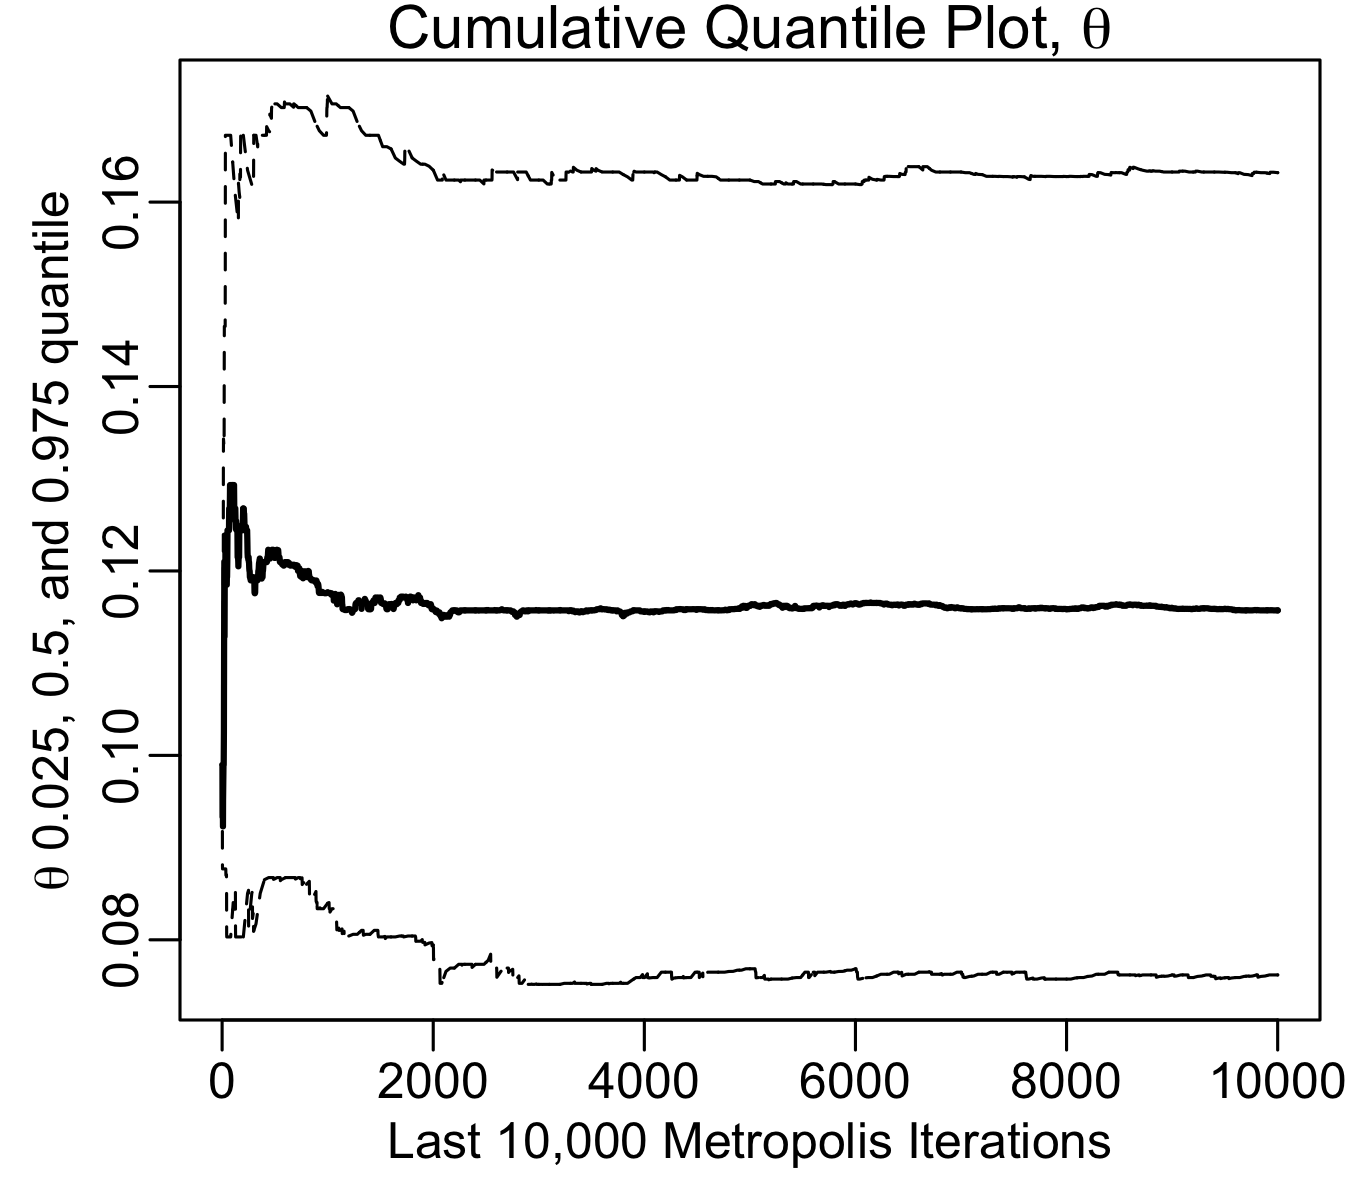
\includegraphics[width=\textwidth]{figures/mcmc_cum_quant_plot_theta.png}
		\caption{}
		\label{fig:quant_theta}
	\end{subfigure}
	\hfill
	\begin{subfigure}[b]{0.49\textwidth}
		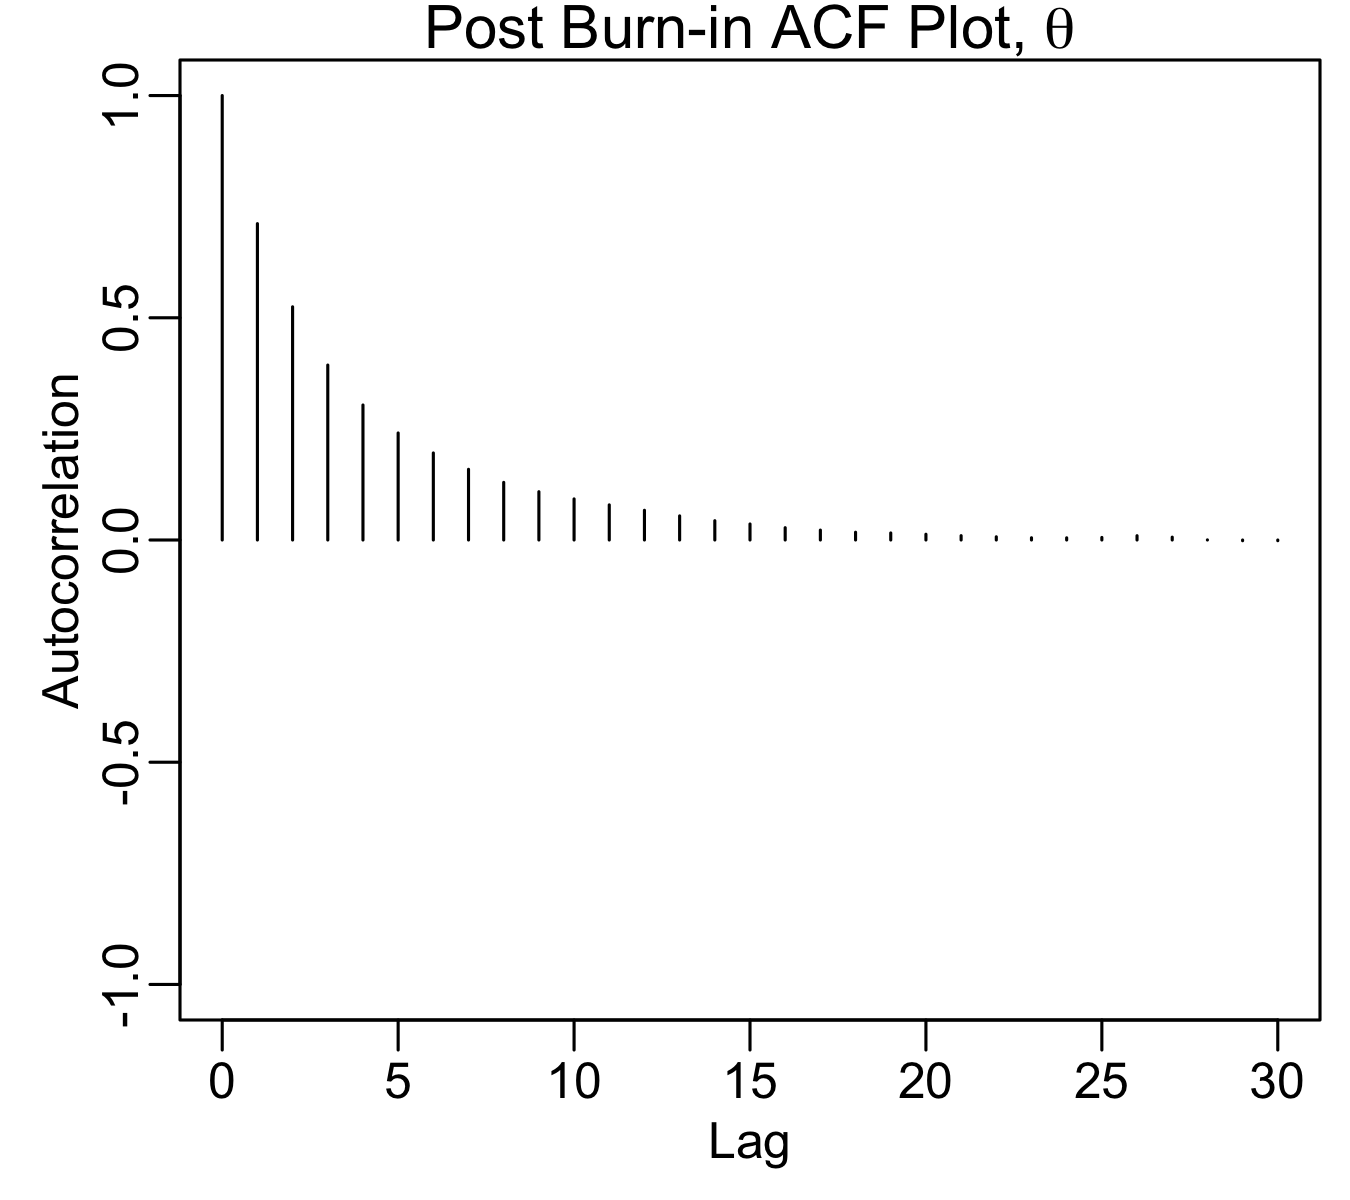
\includegraphics[width=\textwidth]{figures/mcmc_acf_plot_theta.png}
		\caption{}
		\label{fig:acf_theta}
	\end{subfigure}
	\caption{(\subref{fig:quant_theta}) tbd; (\subref{fig:acf_theta}) tbd }
	\label{fig:data_plot}
\end{figure} 

\newpage
\section{Coding Error}
\label{coding_error}

While \citet{Brown} presents several variations of the basic and parallel Metropolis algorithms that improve performance, the authors ultimately determined that the statistical model specified was incapable of capturing the underlying complexities of the plantation data. 
After deriving the parameters for the prior on $\mu$ and simulating epidemics from a subsample of the data, it became clear that the findings reported in \citet{Brown} were based on a irreparably flawed Metropolis algorithm implementation. 
The coding errors were replicated across all implementations and ultimately led the authors to unsupportable conclusions.

Coding the MCMC algorithm as suggested in \citet{Brown} led to run times many orders of magnitude slower than the times reported. 
Running times were prohibitively slow even after taking a 10\% sample of the full data set. 
While this is to be expected for the R prototype, Julia benchmarks against the C programming language indicate that the performance difference cannot be fully explained by the choice of programming language. 
Each method was coded according to standard software engineering best practices, including modular programming and test-driven development approach.  

Simulating new epidemics from the posterior parameters conditioned on the infection intervals and from the posterior parameters alone led \citet{Brown} to the results in figure \ref{fig:post_sim_plot}. 
Comparing the published simulated epidemics based on posterior samples for the number of new infections per week conditioned on the six observations with simulated epidemics based on the posterior parameters without reference to the data shows that the unconditional simulated outbreaks begin much faster than what the data supports. 
This result is completely determined by the endemic infection rate, $\mu$. 
Now, time to the first infection is distributed as an exponential random variable with rate $\mu$. 
If $\mu$ were somehow overestimated, then the time to the first infection would drop substantially.
In this case, the mismatch between the conditional and unconditional simulations in figure \ref{fig:post_sim_plot} are due to an error in the Metropolis sampler. 
Instead of using weakly informative prior $\mu \sim \Gamma(0.7, \text{rate}=0.004)$ with mean 175 and variance $\frac{0.7}{0.004^2}=43,750$, \citep{Brown} specified $\mu \sim \Gamma(0.7, \text{scale}=0.004)$ with mean 0.0028 and variance $1.12\times10^{-5}$. 
As a result, it is clear from figure \ref{fig:prior_mu_plot} that the posterior samples for $\mu$ only reflects the influence of the prior. 
After reviewing the authors' source code, it was confirmed that the authors did in fact use the scale parameterization for all gamma priors in the sampler. 
As a result, $\sigma$ is the only prior properly encoded. 

\begin{figure}[H]
\centering
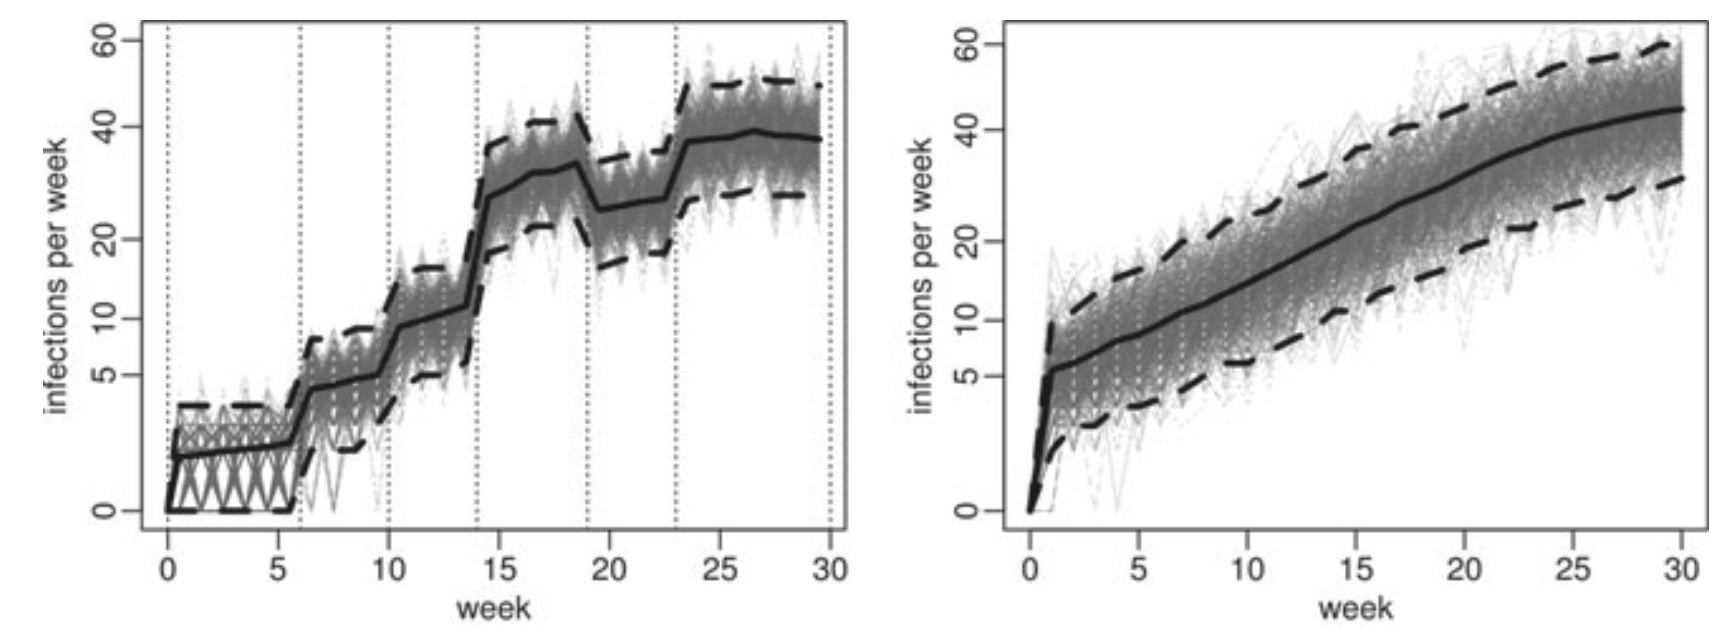
\includegraphics[height=0.36\linewidth, keepaspectratio]{figures/brown_figure_4.png}
\caption{(left) simulated number of new infections per week conditioned on infection times and (right) simulated number of new infections per week simulated from posterior parameters published in  \citet{Brown} }
\label{fig:post_sim_plot}
\end{figure} 

\begin{figure}[H]
\centering
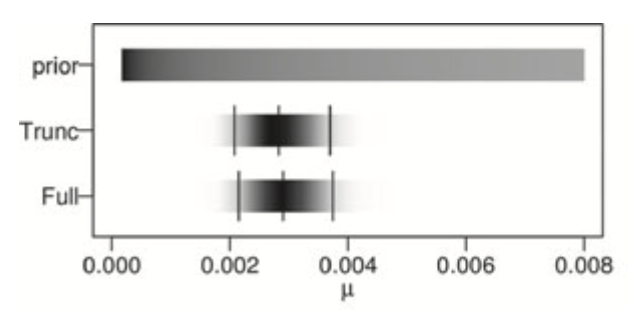
\includegraphics[height=0.26\linewidth, keepaspectratio]{figures/brown_figure_2a.png}
\caption{Range of $\mu$ prior, truncated posterior sample $\mu$, and posterior sample $\mu$ published in \citet{Brown}}
\label{fig:prior_mu_plot}
\end{figure} 


\end{document}


